\documentclass{article}
% Packages used
% Packages
\usepackage{amssymb,amsmath,amsthm,bbm}
\usepackage{verbatim,float,url,dsfont}
\usepackage{graphicx,subfigure,psfrag}
\usepackage{algorithm,algorithmic}
\usepackage{mathtools,enumitem}
\usepackage{multirow}
\usepackage{ragged2e}
\usepackage{xr-hyper}
\usepackage{array}

\usepackage[colorlinks=true,citecolor=blue,urlcolor=blue,linkcolor=blue]{hyperref}
\usepackage[margin=1in]{geometry}
\usepackage[round]{natbib}

\usepackage[utf8]{inputenc} % allow utf-8 input
\usepackage[T1]{fontenc}    % use 8-bit T1 fonts
\usepackage{booktabs}       % professional-quality tables
\usepackage{nicefrac}         % compact symbols for 1/2, etc.
\usepackage{microtype}      % microtypography
\usepackage{pdflscape}

\ifdefined\TimesFont 
\usepackage{times} % use times font
\fi

\ifdefined\ParSkip 
\usepackage{parskip} % use par skip
\fi

% Place page number
\def\fillandplacepagenumber{%
 \par\pagestyle{empty}%
 \vbox to 0pt{\vss}\vfill
 \vbox to 0pt{\baselineskip0pt
   \hbox to\linewidth{\hss}%
   \baselineskip\footskip
   \hbox to\linewidth{%
     \hfil\thepage\hfil}\vss}}
     
% Theorems and such
\newtheorem{theorem}{Theorem}
\newtheorem{lemma}{Lemma}
\newtheorem{corollary}{Corollary}
\newtheorem{proposition}{Proposition}
\theoremstyle{definition}
\newtheorem{remark}{Remark}
\newtheorem{definition}{Definition}

% Assumption
\newtheorem*{assumption*}{\assumptionnumber}
\providecommand{\assumptionnumber}{}
\makeatletter
\newenvironment{assumption}[2]{
  \renewcommand{\assumptionnumber}{Assumption #1#2}
  \begin{assumption*}
  \protected@edef\@currentlabel{#1#2}}
{\end{assumption*}}
\makeatother

% Widebar
\makeatletter
\newcommand*\rel@kern[1]{\kern#1\dimexpr\macc@kerna}
\newcommand*\widebar[1]{%
  \begingroup
  \def\mathaccent##1##2{%
    \rel@kern{0.8}%
    \overline{\rel@kern{-0.8}\macc@nucleus\rel@kern{0.2}}%
    \rel@kern{-0.2}%
  }%
  \macc@depth\@ne
  \let\math@bgroup\@empty \let\math@egroup\macc@set@skewchar
  \mathsurround\z@ \frozen@everymath{\mathgroup\macc@group\relax}%
  \macc@set@skewchar\relax
  \let\mathaccentV\macc@nested@a
  \macc@nested@a\relax111{#1}%
  \endgroup
}
\makeatother

% Min and max 
\DeclareMathOperator*{\argmin}{argmin}
\DeclareMathOperator*{\argmax}{argmax}
\DeclareMathOperator*{\minimize}{minimize}
\DeclareMathOperator*{\maximize}{maximize}
\DeclareMathOperator*{\find}{find}
\DeclareMathOperator{\st}{subject\,\,to}

% Other operators
\DeclareMathOperator{\Cov}{Cov}
\DeclareMathOperator{\Var}{Var}
\DeclareMathOperator{\dm}{dim}
\DeclareMathOperator{\col}{col}
\DeclareMathOperator{\row}{row}
\DeclareMathOperator{\nul}{null}
\DeclareMathOperator{\rank}{rank}
\DeclareMathOperator{\nuli}{nullity}
\DeclareMathOperator{\spa}{span}
\DeclareMathOperator{\sign}{sign}
\DeclareMathOperator{\supp}{supp}
\DeclareMathOperator{\diag}{diag}
\DeclareMathOperator{\aff}{aff}
\DeclareMathOperator{\conv}{conv}
\DeclareMathOperator{\dom}{dom}
\DeclareMathOperator{\tr}{tr}
\DeclareMathOperator{\df}{df}

% Other shortcuts 
\def\R{\mathbb{R}}
\def\C{\mathbb{C}}
\def\E{\mathbb{E}}
\def\P{\mathbb{P}}
\def\T{\mathsf{T}}
\def\half{\frac{1}{2}}
\def\df{\mathrm{df}}
\def\hy{\hat{y}}
\def\hf{\hat{f}}
\def\hmu{\hat{\mu}}
\def\halpha{\hat{\alpha}}
\def\hbeta{\hat{\beta}}
\def\htheta{\hat{\theta}}
\def\indep{\perp\!\!\!\perp}
\def\th{^{\textnormal{th}}}

\def\cA{\mathcal{A}}
\def\cB{\mathcal{B}}
\def\cD{\mathcal{D}}
\def\cE{\mathcal{E}}
\def\cF{\mathcal{F}}
\def\cG{\mathcal{G}}
\def\cK{\mathcal{K}}
\def\cH{\mathcal{H}}
\def\cI{\mathcal{I}}
\def\cL{\mathcal{L}}
\def\cM{\mathcal{M}}
\def\cN{\mathcal{N}}
\def\cP{\mathcal{P}}
\def\cS{\mathcal{S}}
\def\cT{\mathcal{T}}
\def\cW{\mathcal{W}}
\def\cX{\mathcal{X}}
\def\cY{\mathcal{Y}}
\def\cZ{\mathcal{Z}}

 \def\given{\, \vert\, }

\def\TimesFont{} 
\graphicspath{{gfx/}}

\newcommand{\beginsupplement}{
  \setcounter{table}{0}  
  \renewcommand{\thetable}{S\arabic{table}} 
  \setcounter{figure}{0} 
  \renewcommand{\thefigure}{S\arabic{figure}}
  \setcounter{section}{0} 
  \renewcommand{\thesection}{S\arabic{section}}
}
\font\supptitlefont=cmr12 at 16pt 
\newcommand{\attn }[1]{\textcolor{red}{ATTN: #1}}
     
\begin{document}
\title{Retrospective estimation of latent COVID-19 infections before Omicron in the \US}
\author[a,1]{Rachel Lobay}
\author[b]{Maria Jahja}
\author[c]{Ajitesh Srivastava}
\author[d]{Ryan J.\ Tibshirani}
\author[a]{Daniel J.\ McDonald}

\affil[a]{Department of Statistics, The University of British Columbia}
\affil[b]{Department of Statistics \& Data Science, Carnegie Mellon University}
\affil[c]{Department of Computer and Electrical Engineering, University of Southern California}
\affil[d]{Department of Statistics, The University of California, Berkeley}

\footnotetext[1]{To whom correspondence should be
  addressed. E-mail: \email{rachel.lobay@stat.ubc.ca}} 



\date{Version: \today}
\maketitle

\begin{abstract}
The true timing and magnitude of COVID-19 infections are of interest to both the public and to public health, but these are
challenging to pin down for a variety of data-driven and methodological reasons.
Accurate estimates of latent COVID-19 infections can improve our understanding
of the size and scope of the pandemic and provide more meaningful and timely
quantification of disease patterns and burden. In this work, we estimate daily
incident \emph{infections} for each \US state. Rather than taking a model-based
approach, our methods operate directly on data. We first deconvolve reported
COVID-19 cases to their infection date using delay distributions estimated from
the CDC linelist. We combine these deconvolved cases with serology data to scale
up to unreported infections. Our results cover all states at the daily
frequency, incorporate variant-specific incubation periods, and account for
reinfections and waning antigenic immunity. This analysis also produces
estimates for other important quantities such as the number of deconvolved cases
specific to each variant and the infection-case-report ratio. We also discuss some
implications of our results: a disease burden that appears earlier and more
extensively than previously quantified; differential infection-hospitalization
ratio estimates. Our findings help to better understand the impact of the
pandemic in the \US prior to the onset of Omicron and its descendants. 

\end{abstract}

\section{Introduction}
\label{sec:intro}

Reported COVID-19 cases are a staple in tracking the pandemic at varying
geographic resolutions \citep{dong2020interactive, nyt2020corona,
wp2020tracking}. Yet, for every case that is eventually reported to public
health, several infections are likely to have occurred, and likely much earlier.
To see why, it is important to understand \emph{whose} cases are being reported
and what differentiates them from unreported cases as well as \emph{when} these
case reports happen. \Cref{fig:chain_events_onset_report} shows an idealized
path of a symptomatic infection that is eventually reported to public
health. This figure illustrates a number of sources of bias in the
reporting pipeline. For instance, diagnostic testing mainly targets symptomatic
individuals; thus, infected individuals exhibiting little to no symptoms are
omitted \citep{cdc2022estimated}. In addition, testing practices, availability,
and uptake vary temporally and spatially \citep{pitzer2021impact,
ecdc2020strategies, hitchings2021usefulness}. Finally, cases provide a belated
view of the pandemic's progression, because they are subject to delays due to
the viral incubation period, the speed and severity of symptom onset, laboratory
confirmation, test turnaround times, and eventual submission to public health
\citep{pellis2021challenges, wash2020dash}. For these reasons, reported cases
are lagging indicators of the course of the pandemic. Furthermore, they do not
represent the actual number of new infections that occur on any given day based on
exposure to the pathogen. Since there was no large-scale surveillance effort in
the United States that reliably tracked symptom onset, let alone infection
onset, ascertaining the onset of all \emph{infections} is challenging.

\begin{figure}[H]
\centering
    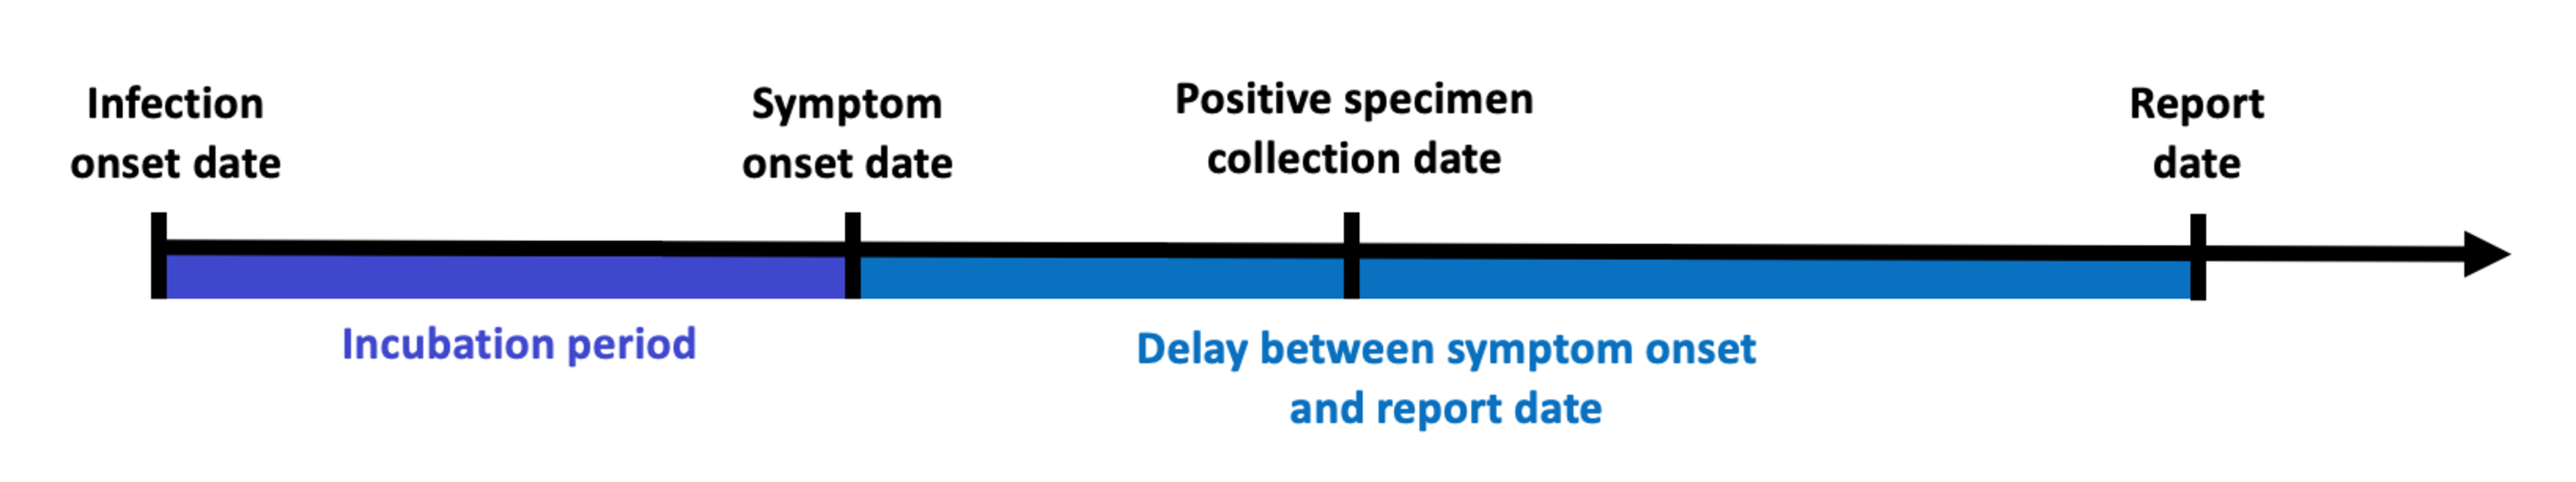
\includegraphics[width=.99\textwidth]{Chain_of_events_onset_report.pdf} 
    \caption{Idealized chain of events from infection onset to case report date 
    for a symptomatic infection that is eventually reported to public health.}
    \label{fig:chain_events_onset_report}
\end{figure}

% Importantly, all of these issues that are present in local health authority
% data are also present in the gold standard for case data from the JHU CSSE
% \citep{dong2020interactive, guidotti2022worldwide} because JHU scrapes case
% data from the local health authority dashboards \citep{jahja2022real}.
% Furthermore, the cases shown on the JHU CSSE Coronavirus Resource Center
% \citep{jhucsse2020covid} are those that have been disseminated to the public
% on a given day. 
% Our approach to estimate latent infections takes case data and estimates the 
% following...

Contextualizing the course of the pandemic, understanding the effects of
interventions, and drawing insights for future pandemics is challenging because
the spatial and temporal behaviour of infections is unknown. While reported
cases provide a convenient proxy of the disease burden in a population, it is
incomplete, delayed, and misrepresents the true size and timing of the pandemic.
Regardless of these difficulties, it is important to the public and to public
health to perform a pandemic post-mortem. Estimates of daily incident infections
are one such way to measure this and can guide understanding of the pandemic
burden over space and time. 

\begin{figure}[H]
\centering
    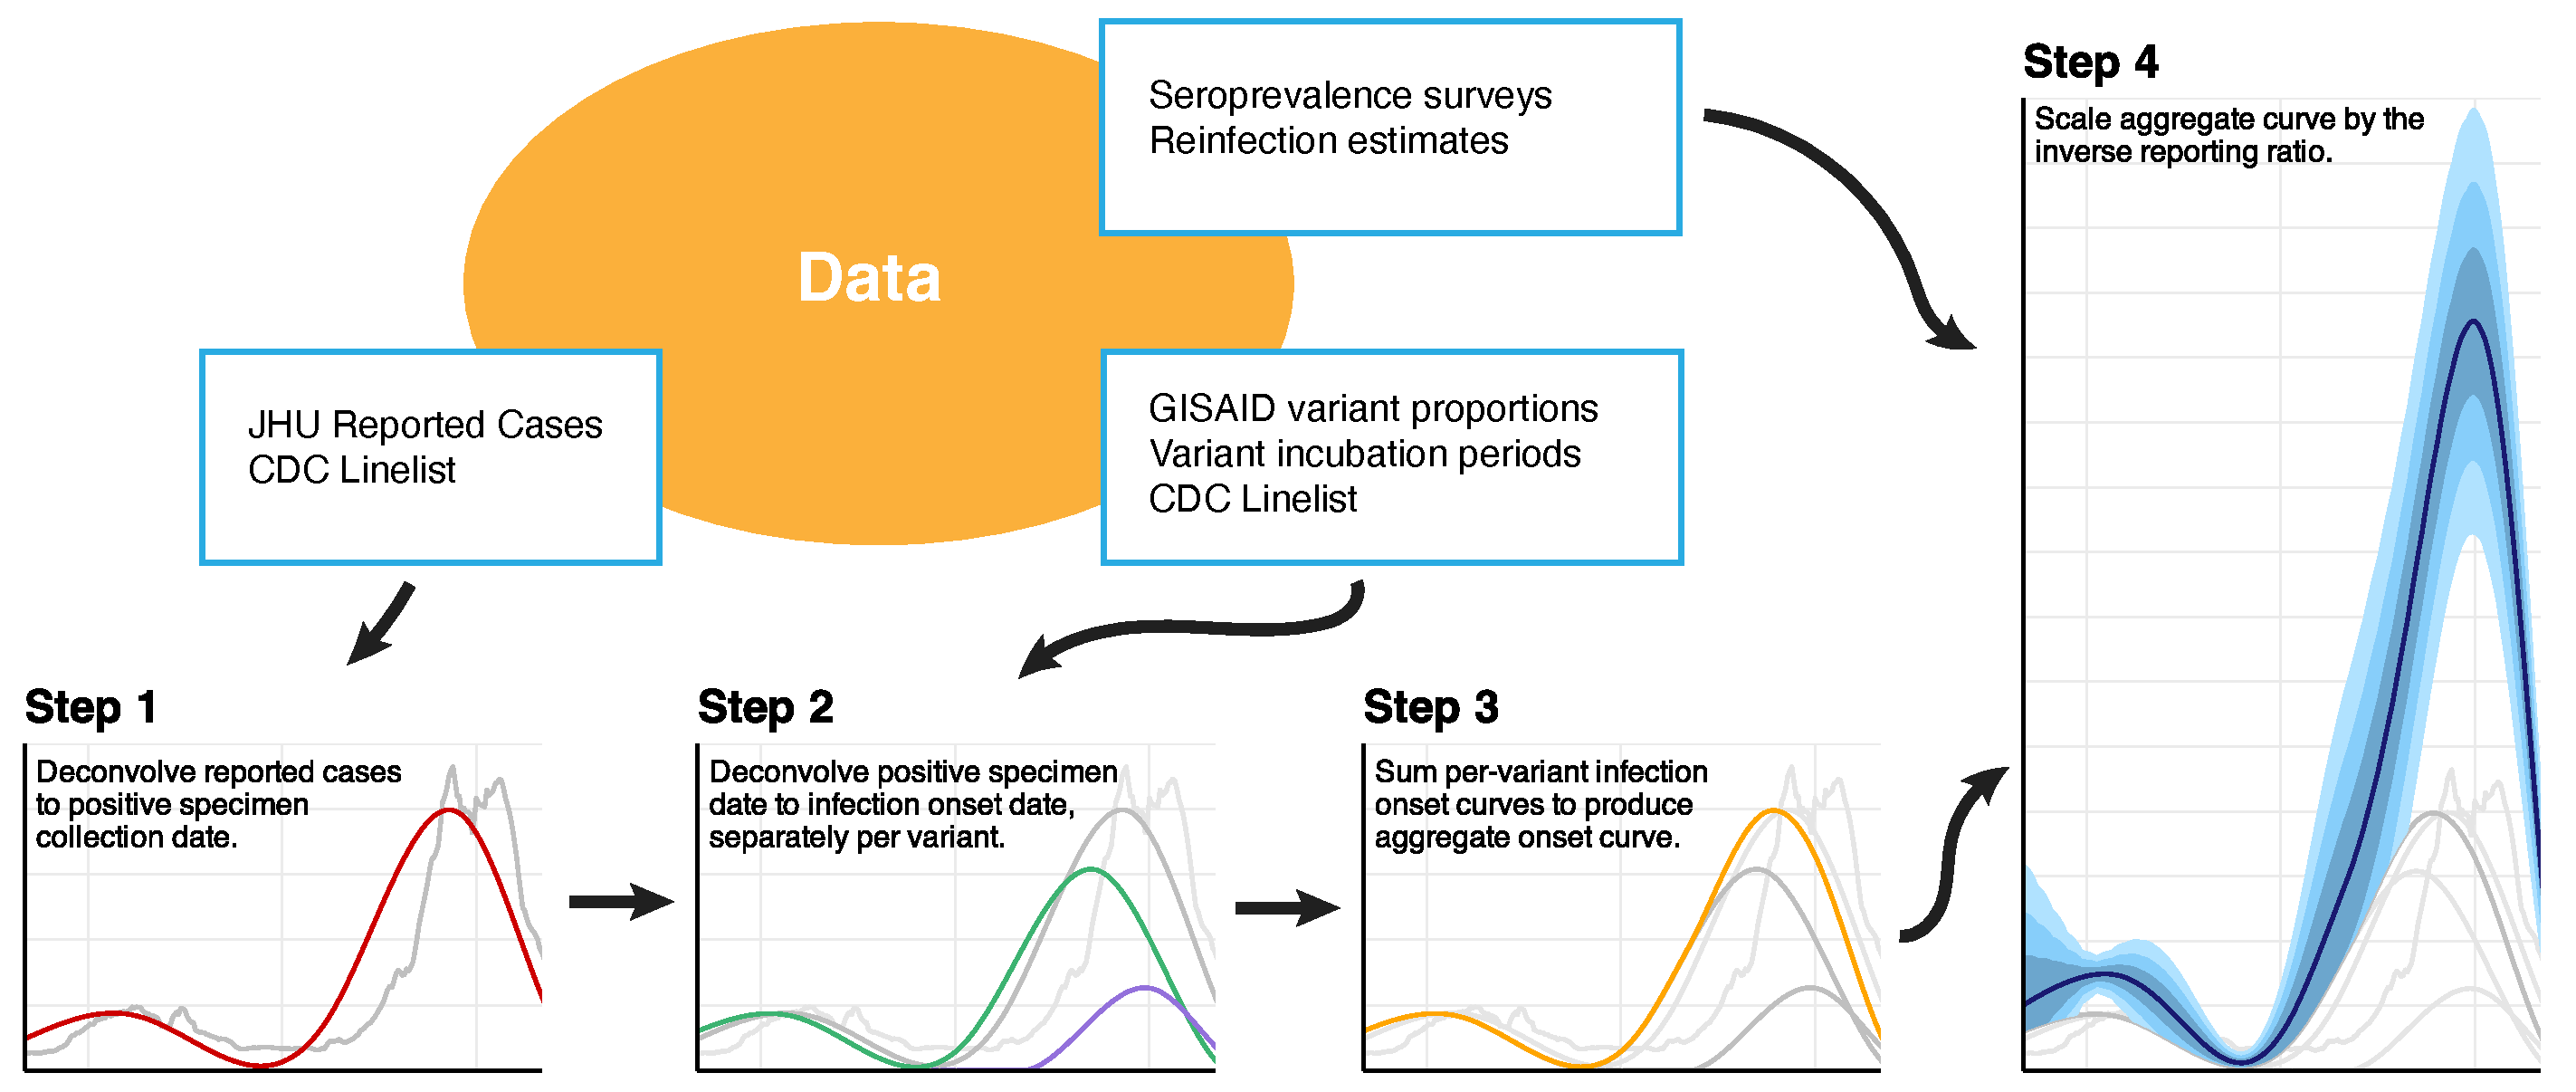
\includegraphics[width=.9\textwidth]{li-flowchart.pdf} 
    \caption{Flowchart of the data and major analysis steps required to get from
    reported cases to incident infection estimates. In Step 1, we use the CDC
    line list data to deconvolve reported cases (grey) backward to the date of
    positive specimen (red). Step 2 separately deconvolves these to the date of
    infection by variant (Epsilon in Purple, Ancestral in Green), 
    before summing across all variants (orange)
    in Step 3. Finally, we use seroprevalence
    survey and time-varying reinfection data to account for the unreported
    infections.}
    \label{fig:cases_to_infect_flowchart}
\end{figure}
    

In this work, we provide a data-driven reconstruction of daily incident
infections for each \US state before the onset of Omicron. Using
state-level line list data, we estimate state-date specific distributions for
the delay from symptom onset to positive specimen date and positive specimen to
case report date. We combine these with variant-specific incubation period
distributions to deconvolve daily reported COVID-19 cases back to their
infection onset, removing the effects of the delays. Finally, we adjust for
unreported infections with seroprevalence and reinfection data, accounting for
the waning of antigenic immunity over time. A graphical depiction of our
procedure is shown in \Cref{fig:cases_to_infect_flowchart}. Our results examine
features of our infection estimates and the implications of using them, rather
than reported cases, to assess the impact of the pandemic. We also produce
simple time-varying infection-hospitalization ratios (IHRs) for each state and
compare these with case-hospitalization ratios (CHRs). While these analyses
provide a glimpse into the utility of our infection estimates, we believe that
there is much more to be explored, and we hope that our work serves as a
benchmark for future retrospective analyses. 



\section{Results}
\label{sec:results}

By estimating the time series of COVID-19 infections per 100,000 inhabitants
for each \US state from June 1, 2020 to November 29, 2021, we observe rates of
infections that vary in intensity and disease burden across space and time
(\Crefrange{fig:state_infect_est}{fig:six-states}). Outbreaks in
infections precede those in cases and are consistently larger in magnitude
(we will use ``cases'' to mean ``reported cases'').

The largest per-capita outbreaks prior to Omicron were observed in the late
summer or early fall of 2021 in Louisiana, Georgia, Idaho, and Montana matching
the intuition that clusters of geographically proximate states are likely to
exhibit similar viral spread. During this time, the two states that have the
highest rate of infections on single day are Louisiana (476 infections per 100K,
on July 20, 2021, 2021) and Idaho (also 457 infections per 100K, on September 7,
2021). The period of lowest viral transmission is observed in the summer of
2020. From June 2020 to the end of August, Vermont saw less than 10 infections
per 100K per week, the longest such lull for any state.



\subsection{Infection estimates reveal waves missed by reported cases}
\label{sec:omitted-waves}

Relative to reported cases, examining estimated infections reveals a rather
different pattern. \Cref{fig:state_infect_est} shows estimates of the number of
daily new infections per 100,000 inhabitants for each \US state from June 1,
2020 to November 29, 2021 compared with reported cases. 

Nearly all states exhibit at least two major waves of infections---the first
begins in the fall of 2020 and extends into the winter season, while the second
starts in the late summer of 2021 and proceeds into mid-fall. These
represent major waves driven by the Ancestral and Delta variants, respectively.
In general, greater similarities in the strength and magnitude of outbreaks
emerge in small clusters of states that border each other. For instance, in the
Western states of Idaho and Montana or in the Southern states of North and South
Carolina the crests and troughs in the waves of infections appear in sync with each
other. Compared to the other states, consistently low rates of infections are
attained in the Northeastern states of Vermont, New Hampshire, and Maine, even
during the aforementioned Ancestral and Delta waves.

While the major Ancestral, Alpha, and Delta waves tend to be visible for most
states, there are clear outbreaks in unreported infections that are not easily
detectable from cases alone in the falls of 2020 and 2021. For example, a wave
of infections is evident in North Dakota and South Dakota over the spring of
2021 that is virtually undetectable from the reported cases. In the late summer
of 2021, the Delta wave is only faintly detectable from cases in a number of
Northeastern states (New York, Massachusetts, Connecticut, and New Hampshire),
and yet the infections suggest that it has already begun in earnest. 

\subsection{The cases-to-infections ratio varies by state and variant}
\label{sec:case-infection-ratio}

\begin{figure}[!tb]
\centering
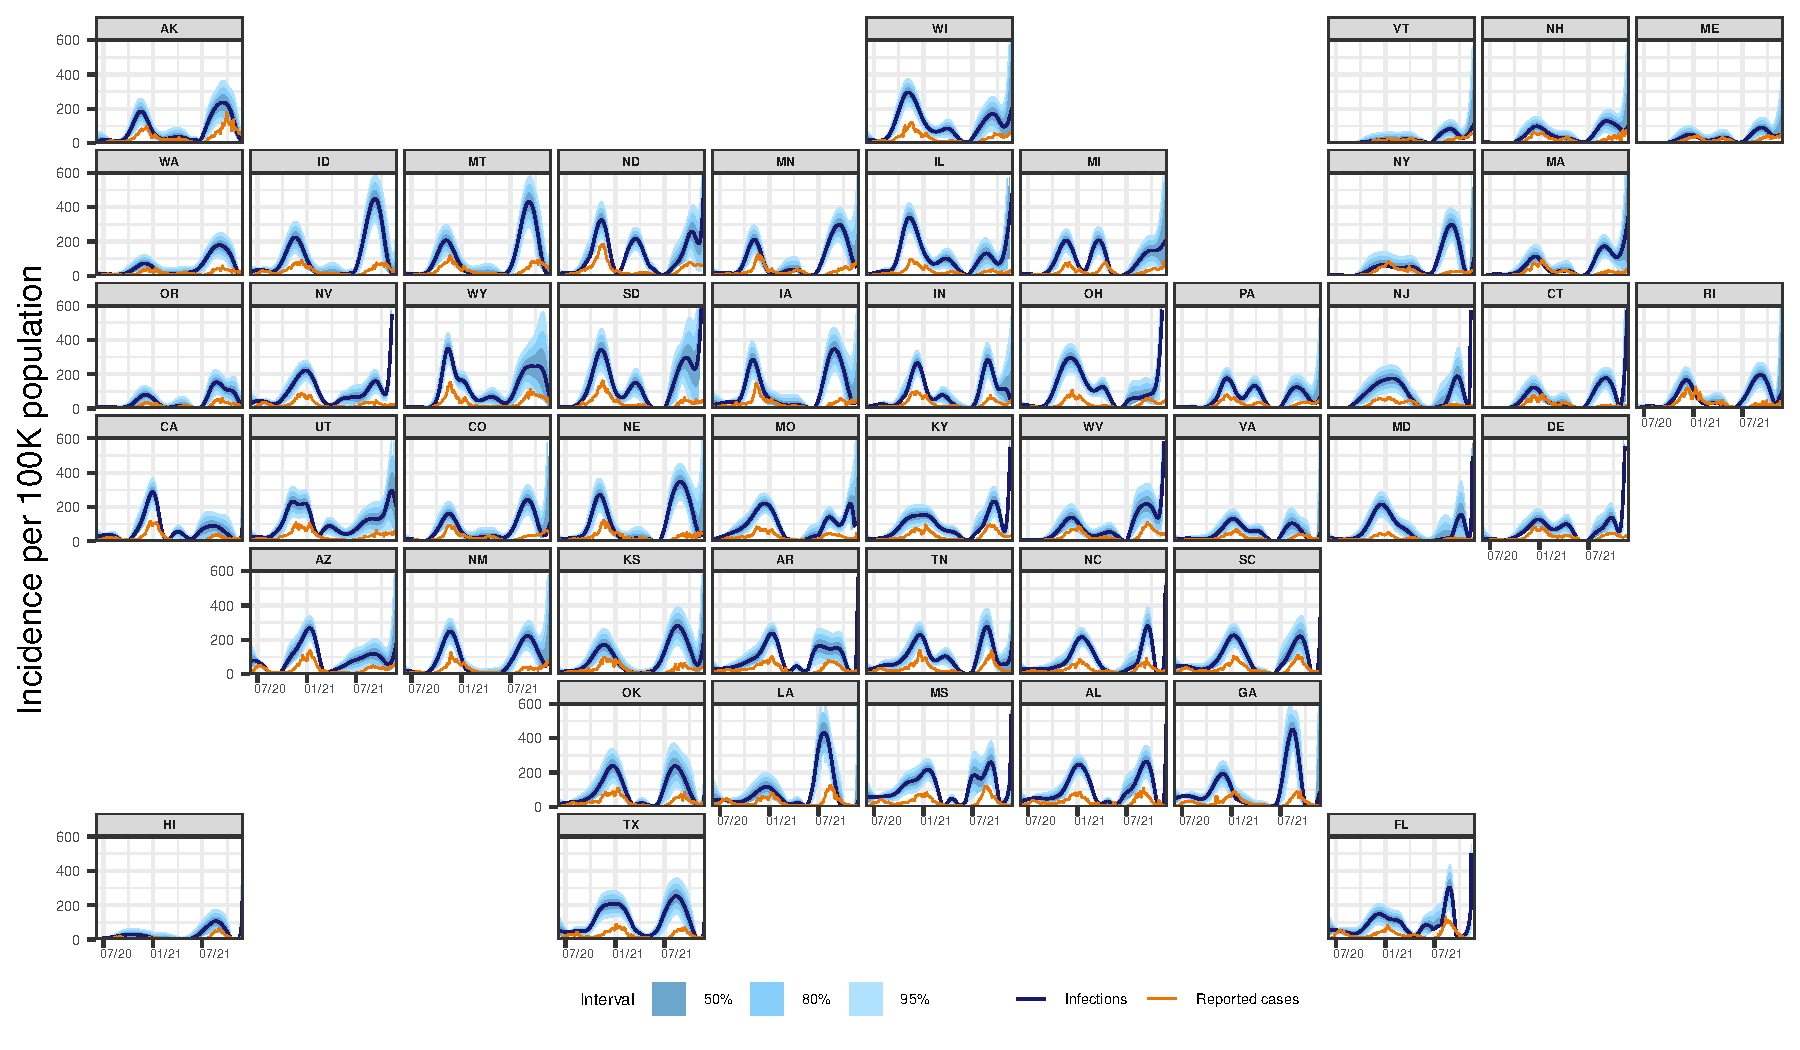
\includegraphics[width=.99\linewidth]{adj-unadj-cases-plot-1.pdf} 
\caption{Estimates of the number of daily new infections per 100,000 population
for each \US state from June 1, 2020 to November 29, 2021 (dark blue line). The
blue shaded regions depict the 50, 80, and 95\% intervals for the estimates,
while the orange line represents the trailing 7-day average of reported cases
per 100,000.}
\label{fig:state_infect_est}
\end{figure}    

While it is clear from \Cref{fig:state_infect_est} that cases underestimate the
true burden of infections for every state, the degree to which this problem
persists varies widely across states and variants. For the Ancestral wave, the
largest discrepancies are more frequently in the Midwest: states such as
Illinois, Indiana, and Ohio. For the Delta wave, some of the largest
discrepancies between cases and infections are visible in the Western states of
Idaho and Montana, the Southeastern states of Louisiana and Georgia, and the
Midwestern states of Iowa and Nebraska. Early in the pandemic, such
discrepancies between cases and infections may be attributable to state-specific
issues with the reporting pipeline, while later, they more likely due to the
rise in asymptomatic infections across variants \citep{oph2022covid,
garrett2022high}. 

The ratio of cases to infections decreases with time. While the Delta wave is
somewhat apparent from the case counts for all states
(\Cref{fig:state_infect_est}), infection estimates suggest that case counts
severely underestimate infections during this period for many states, more so
than in earlier waves. The most extreme was New Jersey, where about 6.3\% of
estimated infections were eventually reported as cases. Similarly low are
Maryland (7.3\%), and Nevada (8.4\%), and South Dakota (10.0\%). This issue
extends to most states: in 44 states fewer than 30\% of infections eventually
appear in case reports. The case-report ratio was larger in earlier waves, and
its effects most apparent in different regions. During Alpha, Louisiana had the
lowest ratio of infections to cases (11.9\%) followed by California (13.6\%).
Such patterns are less apparent during the Ancestral wave, where Ohio and
Maryland had the lowest ratio of reported cases to infections at 21.4\% and
21.7\%, respectively. 

\Cref{fig:choro_inf_case_rates} displays the state-level daily new infections
and cases per 100,000 for five dates over June 2020 to November 2021, allowing a
closer examination of their spatial patterns. For instance, it shows
that on June 1, 2020, there is little difference between case and infection
rates across the states, while later on, the differences become more pronounced.
Furthermore, using cases as a proxy for infections can lead to
misunderstandings in the states that are affected and the extent to which they
are affected. For some days, the spatial extent of infections is understated by
cases. For example, on October 20, 2020, while case rates are elevated in a
handful of upper-Midwestern states (namely, North and South Dakota), infection
estimates are elevated to a similar extent in the surrounding states,
emphasizing a wider impact than is indicated by cases. On July 20, 2021, while
the map of case rates shows low and geographically consistent impact, infection
rates reveal that Texas, Louisiana, Georgia, and their neighbors are hotspots at
that time. 

By focusing on states with elevated cases, infection outbreaks may be
overlooked. For instance, on August 27, 2021, Montana and Idaho have some of the
highest infection rates. In contrast, the case rates are unremarkable for these
two states, whereas the highest case rates tend to be localized in the Southeast. However, the opposite occurs as well: on December
17, 2020, Tennessee and California have the highest case rates but infections
are largely similar to other states.

\begin{figure}[!tb]
\centering
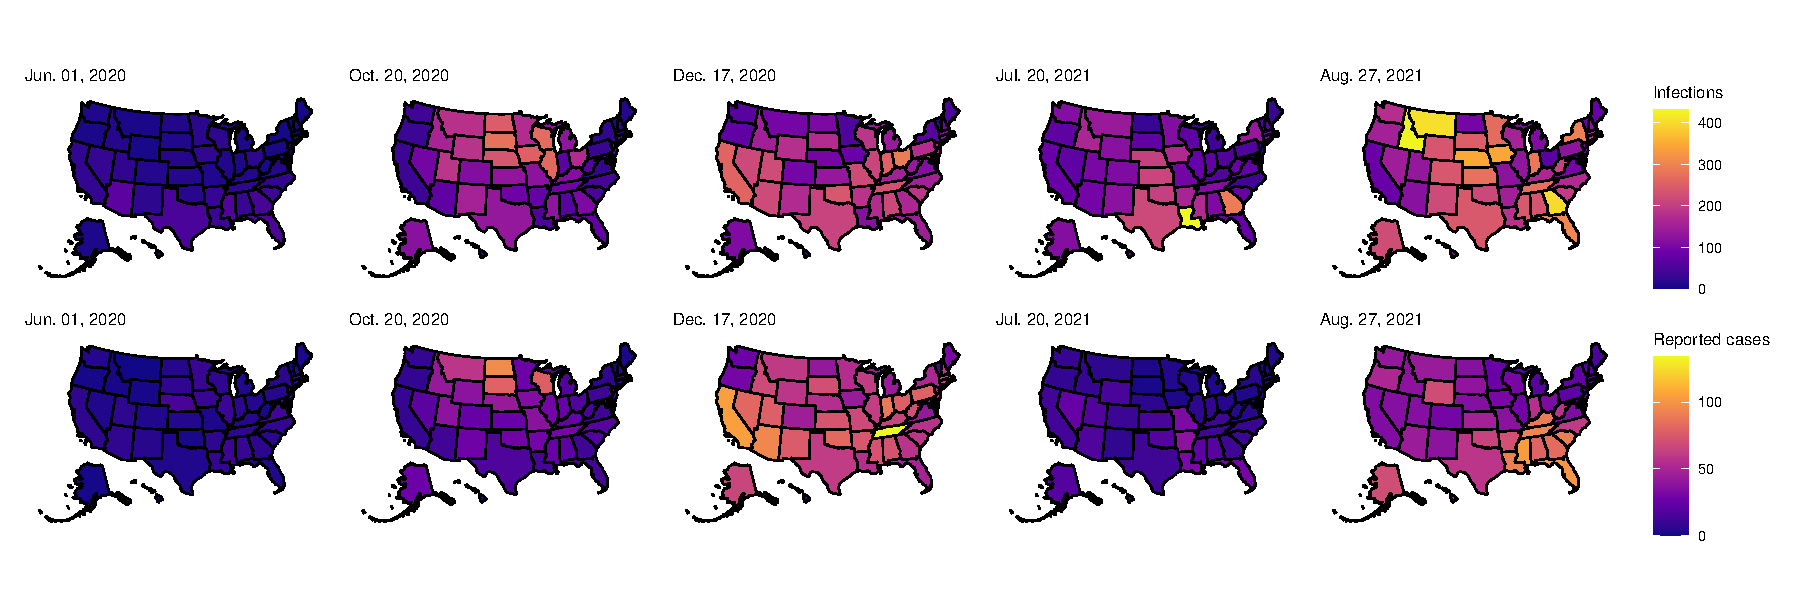
\includegraphics[width=.99\textwidth]{choro-maps-1.pdf}
\caption{Choropleth maps of the state-level estimates of the number of daily new
infections per $100,000$ population (top row) and the daily new cases per
$100,000$ population (bottom row) for five select dates between June 1, 2020 and
November 29, 2021. Note that the first date was chosen as a baseline, while the
other dates were chosen because they show large counts of infections across
all states. In particular, the third and fifth dates present the largest number
of total infections across the 50 states within those calendar years. Note that
the colors are scaled differently for infections and cases to enable relative comparisons.} 
\label{fig:choro_inf_case_rates}
\end{figure}    



    
\subsection{Infections, overall and by variant, emphasize earlier outbreaks}
\label{sec:infections-by-voc}

\Cref{fig:six-states} examines the infection estimates for a selection of states
more closely. The top panel shows infection estimates for these states, while
the bottom panel disaggregates their deconvolved cases based on the locally
circulating variant proportions at the time. These figures show times when the
total infections emphasize earlier outbreaks than are indicated by cases alone.
During the Ancestral wave, infections in Massachusetts, Idaho, Montana,
Louisiana, and Ohio peak earlier than cases. For these states, the infections
peak about 17 days earlier on average, with Massachusetts attaining the maximum
difference of 26 days. Such trends are also observed in the major Delta wave in
the states that present a prominent peak during this time such as Montana and
Louisiana, where infections lead cases by about 41 and 24 days, respectively.
The division by variant categories reveals the variant(s) that are behind these
waves. For example, in California alone, the Epsilon wave appears to coincide
with a second Ancestral wave. To give another example, we can see a
major increase in Alpha in Massachusetts over the spring of 2021. To a lesser
extent, this trend is apparent for all of the other states, save for California,
where Alpha is not a major driver of infections in comparison to the other
variants in circulation around that time. 

\begin{figure}[!tb]
\centering
    \includegraphics*[width=\linewidth]{six-decon-var-1.pdf}
    \caption{Panel A: Reported cases (orange) and estimates of daily new
    infections (dark blue) per 100K inhabitants. The blue shaded regions
    indicate 50, 80, and 95\% confidence bands.  
    Panel B: Deconvolved cases colored by variant per 100K inhabitants.}
    \label{fig:six-states}
\end{figure}


\subsection{Infections lead hospitalizations according to cross-correlations}
\label{sec:lagged-correlations}

We systematically investigate the temporal relationship between infections and
hospitalizations with Spearman's rank-correlation across different lags
(\Cref{fig:correlations}). The maximum average correlation across states is
0.48, occurring at a lag of 13 days. In contrast, we find that the largest
average Spearman correlation for cases is 0.69 and occurs at a lag of 1 day.
That is, case reports are nearly contemporaneous to hospitalizations, while
infection estimates clearly precede them. 

With respect to previous literature, the maximum correlation being attained at a
lag of 13 days is fairly consistent with estimates of the average time from
infection to hospitalization for cases reported in January, 2020 in Wuhan, China
(9.7 days) as well as with estimates from across the pandemic in the UK (ranging
from 8.0 to 9.7 days) \citep{linton2020incubation, ward2021understanding}.
Importantly, our 13 day lag for the \US\ also includes the impact of the
reporting pipeline, a delay omitted from the international estimates. 

\begin{figure}[!tb]
\centering
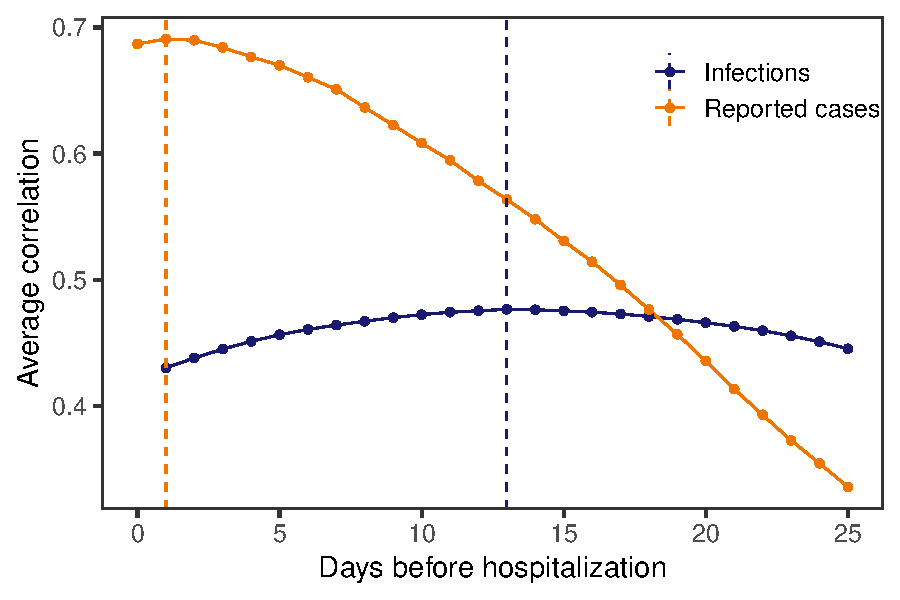
\includegraphics[width=.8\linewidth]{corr-plot-1.pdf} 
\caption{Spearman's rank correlation between each of cases and
infections with hospitalizations per 100,000. These are calculated for each lag,
state, and rolling window of 61 days before averaging. The vertical dashed lines
indicate the lags for which the highest average correlation is attained.}
\label{fig:correlations}
\end{figure}
    

The average correlation is consistently larger for cases than infections (with a
difference of about 0.21 at the peaks). This increase is likely due to two
reasons. First, many cases are detected contemporaneously with hospitalization:
people may first test positive only when they go to to the hospital for
treatment. Second, unreported infections tend to be less severe and less likely
to lead to hospitalization than those that are reported
\citep{sallahi2021using}.



\subsection{IHR estimates tend to be smaller and exhibit less pronounced spikes}
\label{sec:ihrs}

As a counterpart to the correlation analysis, we compute the time-varying
infection-hospitalization ratios (IHRs) for each state using the correlation
maximizing lag (13 days). We similarly compute the case-hospitalization ratios
(CHRs) using their correlation maximizing lag for comparison (1 day,
\Cref{fig:IHR_7dav}). For each state, the CHRs tend to be larger in comparison
to the IHRs. This is consistent with the claim that reported infections are more
likely to require hospitalization than unreported infections. 


\begin{figure}[!tb]
\centering
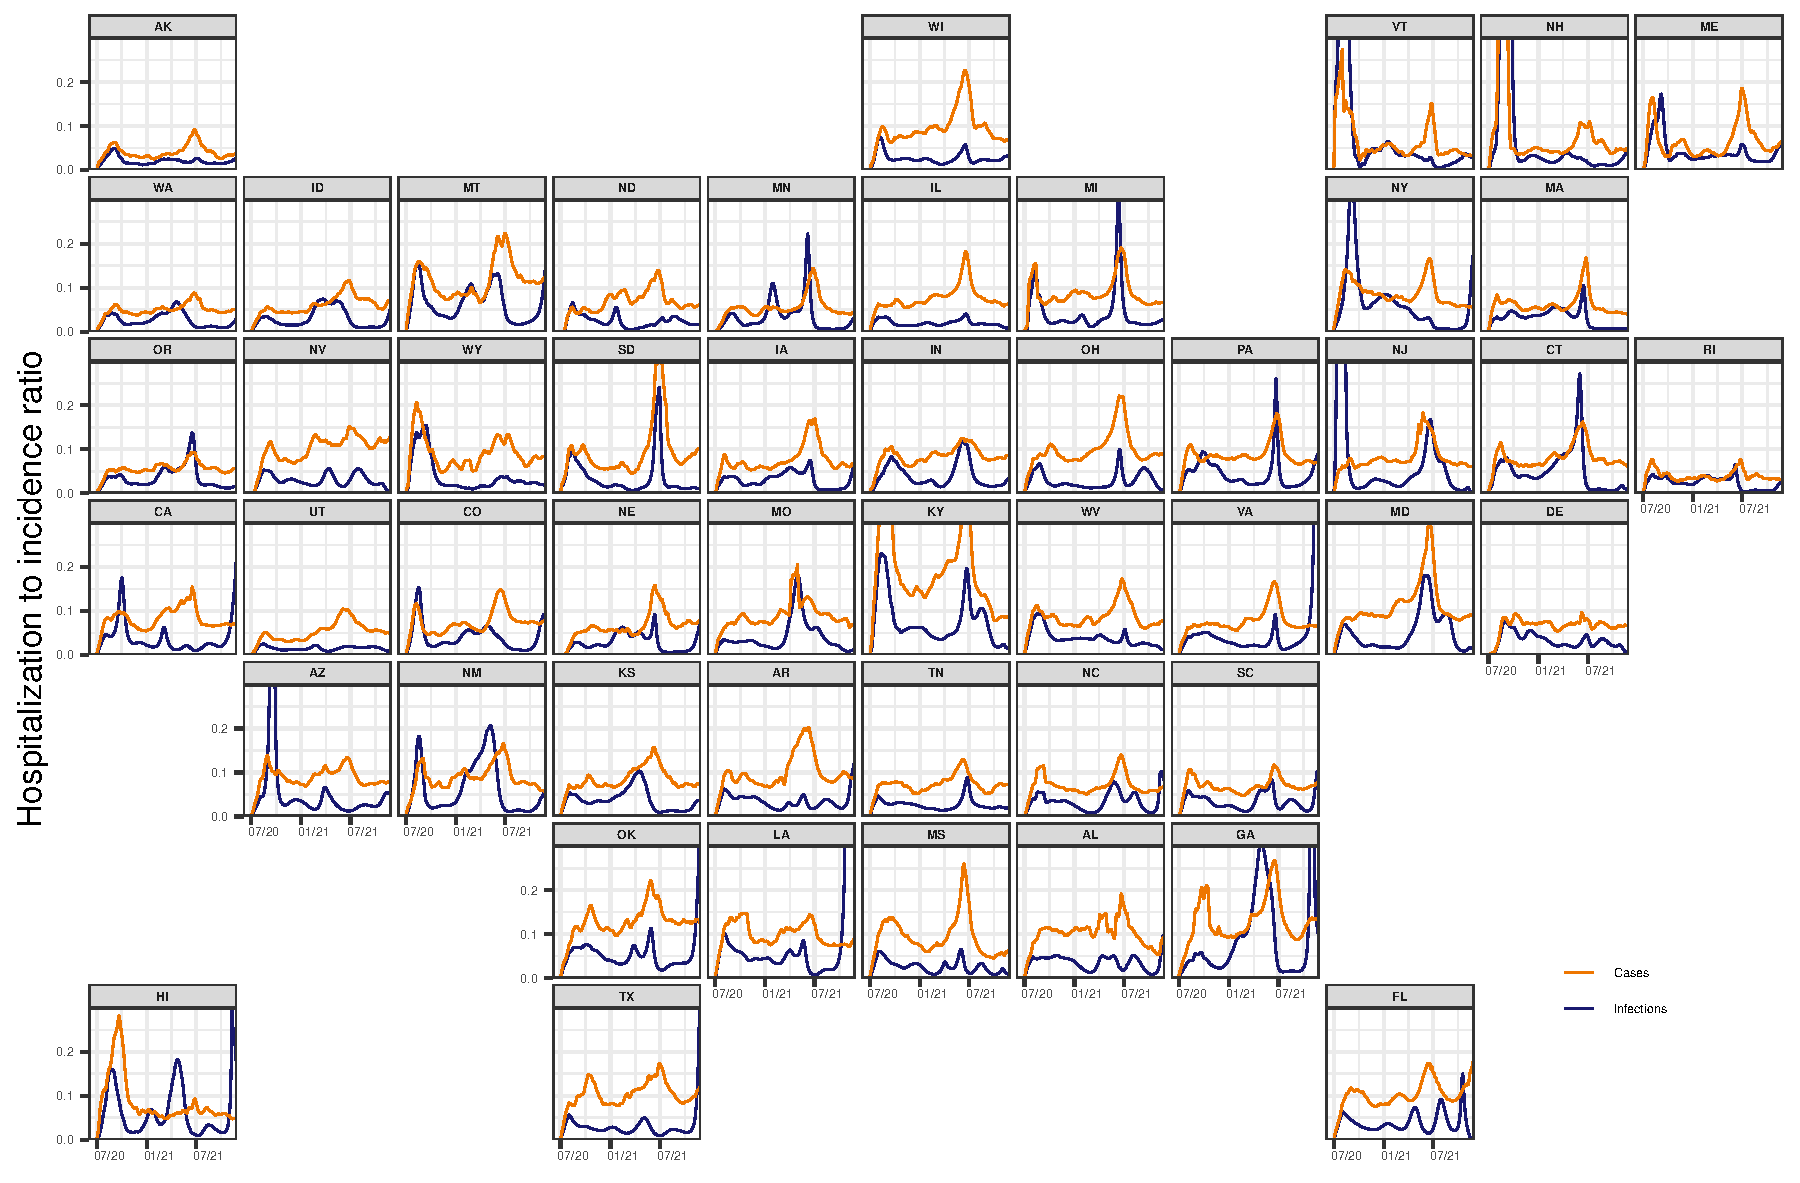
\includegraphics[width=\linewidth]{ihrs-1.pdf}
\caption{Time-varying IHR and CHR estimates for each state from June 1, 2020 to
November 29, 2021, obtained using the respective correlation maximizing lag from
\Cref{sec:lagged-correlations}. Note that the infection, case, and
hospitalization counts are subject to a center-aligned 7-day average to remove
spurious day of the week effects. Also note that the different starting points
across states are due to the availability of the hospitalization data.}
\label{fig:IHR_7dav}
\end{figure}


Both IHRs and CHRs exhibit similar geospatial and temporal trends as those noted
for infections. Namely, states that are proximate (for example, North and South
Carolina) show similar temporal patterns in IHRs and CHRs. In addition, similar
spikes are evident across many states during waves of infections that are driven
by variants of concern. For example, some states exhibit a striking increase in
hospitalizations in mid-2021, which coincides with the rapid takeover of the
Delta variant \citep{hodcroft2021covariants}. This finding aligns with previous
studies that found an increased risk in hospitalization due to Delta
\citep{twohig2022hospital, nyberg2022comparative}. Interestingly, when the
Ancestral variant dominates in 2020, there is a spike in the IHRs that rivals or
sometimes even surpasses that which is observed during Delta. This situation is
most readily observable in New England as well as in some Western states such as
Arizona, New Mexico, and Wyoming.

Overall, the relationship between infections and hospitalizations is
complicated. We observe intermittent spikes that punctuate longer periods where
the IHRs are relatively stable, remaining below 0.1 hospitalizations per
infection. While we computed the IHRs and CHRs for all states, it is important
to note that both likely vary within states and depend on confounding variables
such as age and the presence of major comorbidities
\citep{russell2023comorbidities}. Therefore, it would be beneficial to account
for such variables in their calculations by, for example, stratifying infections
and hospitalizations by age to produce age-specific estimates of the IHRs for
each state~\citep{fox2023disproportionate}.







\section{Discussion}

We retrospectively estimated daily incident infections for each \US state over
the period June 1, 2020 to November 29, 2021. Our estimates suggest, confirming
the intuition, that the pandemic impacted states earlier and at a larger scale
than is indicated by reported cases. They also emphasize that using cases as a
proxy for infections leads to erroneous conclusions about trends in infections.
More importantly, we observe outbreaks in infections that are missed by cases
alone: for example, the Delta wave in New Jersey, Connecticut, and Maryland.
These sorts of omissions serve to emphasize that cases paint an incomplete
picture of the pandemic, especially when outbreaks are largely driven by
unreported infections. Furthermore, since case reports generally follow symptom
and infection onsets, cases have a built-in temporal bias. This bias is in addition
to other biases from differences in reporting across states such as temporary
bottlenecks due influxes of data or more persistent processing issues that
increase the average time from case detection to report \citep{wash2020dash,
dunkel2020covid19}. Thus, while reported cases provide an indication of the
trajectory of the pandemic, it is delayed and incomplete.

Our approach offers a number of advantages. By incorporating state-level case,
line list, and variant circulation data, we are able to construct incubation and
delay distributions that are state- and time- specific. Time-varying and
state-specific seroprevalence data allows the reporting ratio estimates to
similarly vary over space and time, a departure from existing work
\citep{unwin2020state, uga2020covid19}. Unlike previous approaches that use a
single delay distribution to generate estimates for all states
\citep{chitwood2022reconstructing, jahja2022real}, our work avoids this
assumption of geographic invariance, an assumption that is far from realistic
due to differences in reporting pipelines, pandemic response, and variants in
circulation, among other issues. 

Another limitation of previous approaches to estimate infections is that they
often fail to account for reinfections. While reinfections constitute a small
portion of the total infections until the arrival of high immune-escape variants
(BA.1), disregarding them means that the infection-reporting ratio will tend to
be underestimated with seroprevalence data alone. By accounting for reinfections
as well as the waning of seropositivity (\Cref{sec:report-ratio}), we more
accurately estimate this ratio. However, future work could refine this analysis.
Because the waning of immunity is likely to be variant-dependent
\citep{pooley2023durability}, our model's single waning parameter would be more
accurately estimated as a mixture of variant-specific parameters with weights
determined by the proportion of the variants circulating. 
%Relatedly, newer variants may escape detection
%\citep{nih2022assessing, fda2023sars}. While in a retrospective analysis, where
%finalized data is used, this is less likely to be an issue, detection escape
%would pose a problem for real-time estimates of infections.

We chose to end our analysis on November 29, 2021, for two main reasons. The
first is that Omicron and subsequent variants come with substantial increases in
the risk of reinfection in comparison to previous variants, likely due to
increased immune escape \citep{wei2024risk, pulliam2022increased,
eythorsson2022rate}. Access to reinfection data that is representative of each
location under study is paramount for extending the analysis. While it would be
ideal to use the reinfection rates over time for each \US state, many states do
not publicly report reinfection data over the entire time period under
examination, if at all.
% While it would be ideal to use confirmed rates over time for each \US state,
% most states do not publicly report reinfection data over the entire time period
% we considered. So we have turned to suspected reinfection data over time for
% Clark County, USA, as that surveillance is among the most detailed and reputable
% that we have found for the United States. Nevertheless, using such localized
% data raises questions of representativeness and the applicability of such
% estimates to Nevada and all other states. Furthermore, this data has no
% information available beyond suspected third infections, which imposes an
% irremediable bias. However, based on the third infection data available there,
% we expect that the probability of being reinfected more than three times is
% likely very low for time frame considered and so the omission of these would
% impact our infection estimates to a minimal extent. 
%
% The vast majority of issues we encountered when trying to reconstruct the
% infection time series for each state are due to an absence or a lack of data.
% Such is the primary issue we had with the restricted line list. In comparison to
% the number of JHU cases (which we are treating as a gold standard) for the same
% release date, we noted there are about $10$ million cases that are unaccounted
% for in the CDC line list. Moreover, the missingness does not appear to be random
% and uniformly distributed across states. Rather it is unequally distributed,
% suggesting that the dataset is likely biased. However, more information on the
% cases that are missing versus present would be required to determine the extent
% the missing cases led to a nonrepresentative, and therefore, biased sample, and
% could be a topic of further study.
The second reason is that the case-ascertainment ratio after December 2021 can
no longer be estimated with seroprevalence data alone. Specifically, while most
state-level data suggests that reinfections still account for less than 20\% of
reported cases during Omicron \citep{ruff2022rapid, nyreinfect2021,
hireinfect2022, wareinfect2022}, seropositivity rapidly reaches nearly 100\% of
the population. Therefore, alternative data sources for estimating the
case-ascertainment ratio must be considered. For example, wastewater
surveillance data may be complementary to seroprevalence data, especially when
testing is low, or serve as a substitute when it is unavailable
\citep{mcmanus2023predicting}. In follow-up work, we extend our
construction of daily incident infections for some states where sufficient data
is available to track reinfections and to incorporate wastewater data.
% However, viral detection is inconsistent across
% locations due to temperature, per-capita water use, and in-sewer travel time
% \citep{mcmanus2023predicting, hart2020computational, li2023correlation}.
An alternative approach could use surveillance streams such as those from
surveys, helplines, or medical records could potentially be integrated if they
offer a sufficiently strong signal of the disease intensity over time
\citep{reinhart2021open,ecdc2020strategies}.



% \attn{Some into Methods, some into Supplement}
% also runs the risk of being nonrepresentative of the
% intended population \citep{bajema2021estimated}. For example, in the blood donor
% dataset some states have region specific-estimates, which clearly do not stand
% for the entire state. Another source of systematic variation is in the
% characteristics of the individuals who opt for blood tests versus those who do
% not. For instance, there may be a healthy user bias, in which a number of those
% who opt for blood tests are generally more inclined to partake in proactive
% healthy behaviors (such as checking on basic health markers by taking an annual
% blood test) than those who do not \citep{parsley2018blood}. Alternatively, a
% number of individuals may be recommended for blood tests by their doctors due to
% signs of ill-health (ex. mineral deficiencies or underlying medical conditions).
% The extent that each such bias persists depends on the purpose of the blood test
% and whether it was used as a proactive or reactive medical tool. Since such
% information is unavailable to us, all we can conclude is that participant-driven
% sources of bias impact the seroprevalence samples to an undetermined extent.
% There are additional concerns about the performance of antibody testing for
% individuals with mild or asymptomatic disease as well as about the loss of
% immunity over time \citep{kaku2021performance, seow2020longitudinal,
% ibarrondo2020rapid}.
% 
% In this work, we do not attempt to directly address infection underascertainment
% due to the increase in asymptomatic infections across variants
% \citep{pho2023covid19}. We simply note that this would likely pose a greater
% problem later in the pandemic, particularly after the Delta era
% \citep{fan2022sars}. We hope that such infections would be largely represented
% by the seroprevalence and reinfection estimates, but there is undoubtedly
% increasing reliance on such estimates to be able to do this over time (owing to
% the simultaneous decline in the reporting cadence and the apparent rise in
% asymptomatic infections over time) \citep{oph2022covid, garrett2022high,
% blauer2022reduce, ren2021asymptomatic}. Consequently, there is an increasing
% uncertainty over time that is not captured by the model or the estimates.   


Our work develops a deconvolution-based approach to inferring infection onset,
combining available line list data with variant circulation estimates and
literature derived incubation periods. The result removes the effects of the
delay from reported cases, pushing them back to infection onset. This approach
process is complemented with the development of a model that leverages the
measurements of waning detectable antibody levels and seroprevalence surveys.
The resulting infection estimates as well as their geospatial and temporal
trends are strongly grounded in both data and statistical models.
%
% Our approach is predicated upon having case, line list, viral circulation, and
% seroprevalence data for each state, all of which are readily available (or
% available upon request in the case of restricted line list data). As a result of
% this, we are able to demonstrate the feasibility of estimating COVID-19
% infections at the state level by using standard sources of data. 
%
% Our framework is quite versatile as it lends itself to more localized, county or
% community level estimates, or globalized, country-specific estimates.
% Fundamentally, to produce estimates of infections for different geographic
% regions, one would simply need to input the required data and re-run the code
% pipeline. In this way, one could readily adapt our approach to generate
% estimates for the provinces in Canada or the regions in England.
%
These well-informed, localized estimates of COVID-19 infections over time
provide a clearer and more comprehensive understanding of the course of the
pandemic. Such estimates contribute important information on the timing and
magnitude of the disease burden for each location, and they highlight trends
that may not be visible from reported case data alone. Therefore, our infection
estimates provide key information for the ongoing investigation on the true size
and impact of the pandemic.


\section{Methods}
\label{sec:methods}


In what follows, we provide details on how we estimate the daily incident
infections for each state over the considered time period of June 1, 2020 to
November 29, 2021 and the data we used to achieve this.
\autoref{fig:cases_to_infect_flowchart} provides a visual summary of the major
analysis tasks, which can be summarized as follows: First, we estimate the time-varying
delays from positive specimen to report date using a line list and use these
to deconvolve reported cases to the date of the positive specimen collection.
Then, we estimate the delay from symptoms to positive specimen, 
combine this with variant specific
infection-to-symptoms delays, and use this delay to push back to the date
of infection. The resulting infection onset estimates are aggregated
across the variant categories and adjusted to account for the unreported
infections by using state-specific, time-varying seroprevalence data in an
antibody prevalence model. 

\subsection{From reported cases to positive specimen collection}
\label{sec:step1}

Deconvolution ``pushes back'' reported cases to the likely date of positive
specimen collection. An important aspect of our methods is that deconvolution is
not the same as a simple shift, rather it involves the distribution of delays
(specific to each state and date), as estimated from de-identified patient-level
line list data on COVID-19 cases from the CDC \citep{cdc2020caserestr}. Simply
shifting cases back in time would fail to reflect the fact that some cases take
much longer to be reported than others.

We will start by describing how the model for deconvolution infers the likely
dates of positive specimen collection from reported cases before describing how
the line list was used to estimate the necessary delay distribution. Together,
these are the ingredients for Step 1 in \Cref{fig:cases_to_infect_flowchart}.
Define $y_{\ell,t}$ to be the number of new cases reported in location $\ell$ at
time $t$, as reported by the John Hopkins Center for Systems Science and
Engineering (JHU CSSE)\citealp{dong2020interactive} and retrieved with the
COVIDcast API \citep{reinhart2021open}. Let $\pi_{\ell,t}(k)$ be the probability
that these reported cases at time $t$ were collected $k$ days earlier. Then, we
model $y_{\ell,t}$ as Gaussian with mean 
\begin{align}
  \label{eq:cases-model}
  \mathbb{E}[y_{\ell,t} \mid x_{\ell,s}, s \leq t ] =\sum_{k} \pi_{\ell,t-k}(k)x_{\ell,t-k},
\end{align}
a probability weighted sum of the number of positive specimens
collected $k$ days earlier, $x_{\ell,t-k}$.
We estimate $\mathbf{x}_\ell = \{x_{\ell,1},\ldots,x_{\ell,T}\}$ by minimizing
the negative log-likelihood with a penalty that encourages smoothness in time.
Thus, our estimator is given by
\begin{align}
  \label{eq:cases-deconvolved}
  \widehat{\mathbf{x}}_\ell = \argmin_{\mathbf{x}}\ \sum_{t}
  \left( y_{\ell,t} -  \sum_k \pi_{\ell,t-k}(k) x_{t-k} \right)^2 
  + \lambda\ \sum_t \big|x_t - 4x_{t-1} + 6x_{t-2} -4x_{t-3}+ x_{t-4}\big|.
\end{align}
The two parts of this optimization problem trade data fidelity (the sum of
squared errors) with smoothness in the resulting estimates (the fourth order
differences of $\mathbf{x}$). The tuning parameter $\lambda$ determines the
relative importance of these competing goals. The solution to the problem is an
adaptive piecewise cubic polynomial \citep{tibshirani2014adaptive,
tibshirani2022divided} and can be accurately computed with ease
\citep{ramdas2016fast,jahja2022real}. We select $\lambda$ with cross validation
to minimize the out-of-sample reconvolution error. Additional details about
convolution are given in the Supplement, \Cref{supp:convol}.
% with $3$-fold cross validation
% \citep{jahja2022real} in which every third day is reserved for testing, and the
% value that results in the smallest out-of-sample mean squared error is chosen.

%\subsection{Estimating delay distributions from private line lists}
%\label{sec:delaystop}

To estimate the $\pi_{\ell,t}(k)$ for all states $\ell$, times $t$, and delays
$k$, we use the CDC line list \citep{cdc2020casepub,
cdc2020caserestr}. The line list contains three key dates of interest for many
cases that will eventually appear in JHU CSSE case reports: symptom onset,
positive specimen collection, and report to the CDC. Handling missingness and
imputation in these dates requires careful attention, and so additional details and
justifications are provided in the Supplement, \Cref{supp:linelist-details}.
Define $z_{\ell,t}$ to be a case report occurring at time $t$ in
location $\ell$, and let $\pi_{\ell,t}(k)$ be the probability that
$z_{\ell,t}$ has a positive specimen collected $k$ days earlier. We assume that
all positive specimen results will be reported within 60 days and that no test will be
reported on the same date as it was collected; that is, $\pi_{\ell,t}(0) = 0$
and $\pi_{\ell,t}(k) = 0$ whenever $k > 60$, which reduces the estimation task to
$\pi_{\ell,t} = (\pi_{\ell,t}(1), \dots, \pi_{\ell,t}(60))$.
Under these assumptions, let $N_{\ell,t}$ be the total number of
$z_{\ell,r}$ with positive specimen in $[t-75+1, t+60] = \mathcal{S}_t$. 
Then, we compute
\begin{align}
  \label{eq:line-list-delay}
    \tilde{p}_{\ell,t}(k) = \frac{1}{N_{\ell,t}} \big(\textrm{\# $z_{\ell,r}$ with positive specimen at $r-k$}\big).
\end{align}
We compute a similar national quantity $\tilde{p}_{t}(k) =
\frac{1}{N_{t}} \big(\textrm{\# $z_{r}$ with positive
specimen at $r-k$}\big)$, without restricting to location $\ell$. Next, let
$\alpha_{\ell,t}$ be the ratio of $N_{\ell,t}$ to the number of cases reported
by JHU CSSE\cite{dong2020interactive} in the window $[t-60+2, t+75]$. 
Then, compute $p_{\ell,t} = \alpha_{\ell,t}\tilde{p}_{\ell,t} +
(1-\alpha_{\ell,t})\tilde{p}_t$. This construction was adopted to allow for more reliance
on the state estimate when there are more CDC cases relative to JHU (and vice
versa). We calculate the mean $m_{\ell,t}$ and variance $v_{\ell,t}$ of
$\{p_{\ell,t}(k) : 0<k\leq 60\}$ and estimate a gamma distribution by solving
the moment equations $m_{\ell,t} = \alpha_{\ell,t}\theta_{\ell,t}$ and
$v_{\ell,t}= \alpha_{\ell,t}\theta_{\ell,t}^2$ for the shape $\alpha_{\ell,t}$
and scale $\theta_{\ell,t}$. Finally, we discretize the resulting gamma density
to the support set of 1 to 60 days to produce an estimate
$\{\widehat{\pi}_{\ell,t}(k): 0 < k \leq 60\}$ of the delay distribution
$\pi_{\ell,t}$. Additional minor details and justification for the delay 
distribution calculations are deferred to Section \Cref{supp:delay-justifications}.
 
\subsection{From positive specimen collection to infection onset}
\label{sec:step2-and-3}

To continue, pushing positive specimen collection time back to infection onset
(Step 2 in \Cref{fig:cases_to_infect_flowchart}), we will use a procedure very
similar to that described above and specified in
\Crefrange{eq:cases-model}{eq:cases-deconvolved}. However, because
the delays involve the time from infection to symptom onset, these must be
variant-specific. This means that both the probabilities and the observations
must be replaced with variant specific quantities. 

For the observations, we use our estimates from \Cref{sec:step1},
$\widehat{\mathbf{x}}_\ell$, but we weight them corresponding to the mix of
variants in circulation. To estimate the daily proportions of the variants
circulating in each state, we use GISAID genomic sequencing data from
CoVariants.org \citep{hodcroft2021covariants, elbe2017data}, and estimate a
multinomial logistic regression model. This procedure is now standard
\citep{obermeyer2022analysis, annavajhala2021emergence, figgins2021sars}, so we
defer details to the Supplement, \Cref{sec:variant-proportions}. The resulting
estimated probability of variant $j$ is given by $\hat{v}_{j\ell,t}$.

To estimate variant-specific delays from infection to positive specimen
collection, we convolve the location-time-specific symptom-to-test distributions
(that are estimated from the CDC line list in the same way as in \Cref{sec:step1}), 
with variant-specific incubation periods.
The convolution of these yields a distribution $\tau_{j\ell,t}(k)$. 
Details on the convolution and its inputs are deferred to the Supplement, 
\Cref{supp:delay-sops,sec:incubation,supp:details-conv}. 

Analogous to
\Crefrange{eq:cases-model}{eq:cases-deconvolved}, for each variant $j$, we model
the variant-specific, deconvolved cases as Gaussian with mean
\begin{align}
  \mathbb{E}\left[\widehat{v}_{j\ell,t}\widehat{x}_{\ell,t} \mid u_{j\ell,s}, s \leq t  \right] = \sum_k \tau_{j\ell,t-k}(k) u_{j\ell,t-k} 
\end{align}
and estimate $\mathbf{u}_{j\ell}$ by minimizing the negative loglikelihood with
a penalty to encourage smoothness:
\begin{align}
\widetilde{\mathbf{u}}_{j\ell} = \argmin_{\mathbf{u}}\ \sum_{t} 
\left( 
    \widehat{v}_{j\ell,t} \widehat{x}_{\ell,t} -  
    \sum_k \tau_{j\ell,t-k}(k) u_{t-k} 
\right)^2 
+ \lambda\ \sum_{t} \big|u_{t} - 4u_{t-1} + 6u_{t-2} -4u_{t-3}+ u_{t-4}\big|.
\end{align}
We call the solution $\widetilde{\mathbf{u}}_{j\ell}$ the \emph{variant-specific
deconvolved cases} and emphasize that these are cases that will eventually
be reported to public health. Because this deconvolution is done separately for
each location and variant, we add them together at each time $t$, and
we denote the total deconvolved cases at location $\ell$ as
$\widehat{\mathbf{u}}_\ell = \sum_j \widetilde{\mathbf{u}}_{j\ell}$ (Step 3 in \Cref{fig:cases_to_infect_flowchart}). 




\subsection{Inverse reporting ratio and the antibody prevalence model} 
\label{sec:report-ratio}

To capture the unreported infections, it is necessary to adjust these
deconvolved case estimates by the ratio of the true number of new infections to
the new reported infections (Step 4 in \Cref{fig:cases_to_infect_flowchart}). 
Seroprevalence of anti-nucleocapsid antibodies represents the percentage
of people who have at least one resolving or past infection \citep{cdc2020data},
so we use the change in subsequent seroprevalence measurements to estimate
\emph{all} new infections rather than just those eventually appearing as cases.

We use two major contemporaneous surveys to estimate the proportion of the
population with evidence of previous infection in each state over time: the
2020--2021 Blood Donor Seroprevalence Survey and the Nationwide Commercial Lab
Seroprevalence Survey \citep{cdc2021blood, cdc2021comm}. See Supplementary
Methods, \Cref{supp:sero-details} for additional details. Each of these provides
seroprevalence estimates along with confidence intervals. In order to account
for different surveys occurring on different dates with roughly weekly
availability and measurement error, we treat actual seroprevalence $s_{\ell,m}$
as a latent variable available on Monday (using $m$ rather than $t$ to denote
Mondays). Therefore, the observed seroprevalence survey measurements $r^1_m$ and
$r^2_m$ are modelled as Gaussian,
\begin{align}
\label{eq:sero-measurements}
r^1_{\ell,m} \mid s_{\ell,m},\ w^1_{\ell,m} &\sim \textrm{N}(s_{\ell,m},\ w^1_{\ell,m}\sigma^2_{\ell,r}),\\
r^2_{\ell,m} \mid s_{\ell,m},\  w^2_{\ell,m}
  &\sim \textrm{N}(s_{\ell,m},\ w^2_{\ell,m}\sigma^2_{\ell,r}),
\end{align}
with source-specific measurement errors that scale proportional to the reported
confidence intervals, respectively $w^1_{\ell,m}$ and $w^2_{\ell,m}$.  

To complete the model, we suppose that latent seroprevalence is modeled as a
Guassian with mean given by the fraction of the previous seroprevalence
measurement at $m$ plus the reinfection-adjusted deconvolved cases multiplied by
the inverse reporting ratio at time $m$:
\begin{align}
  \label{eq:expect-sero}
\mathbb{E}[s_{\ell,m+1} \mid s_{\ell,m}] & = (1 -\gamma) s_{\ell,m} 
+ a_{\ell,m} (1 - z_{m}) \sum_{t\in[m,m+1]}\widehat{u}_{\ell,t},
\end{align}
where $\widehat{u}_{\ell,t}$ are deconvolved cases (from
\Cref{sec:step2-and-3}), $z_{m}$ is the fraction of reinfections, and
$a_{\ell,m}$ is the inverse reporting ratio. Note that $\gamma$ is the fraction
of people whose level of infection-induced antibodies falls below the detection
threshold between time $t$ and time $t+1$. The daily fraction of new infections
$z_t$ are based on surveillance work conducted by the Southern Nevada Health
District \citep{ruff2022rapid}. These results are broadly similar to those in
other locations with available data  \citep{ruff2022rapid, nyreinfect2021,
hireinfect2022, wareinfect2022}. Finally, we specify the time-varying evolution
of the inverse reporting ratio as Gaussian with expectation,
\begin{align}
  \label{eq:report-ratio}
\mathbb{E}[a_{\ell,m+1} \mid a_{\ell,m},\ a_{\ell,m-1},\ a_{\ell,m-2}] = 3a_{\ell,m} - 3a_{\ell,m-1} + a_{\ell,m-2}.
\end{align}
This construction for \Cref{eq:report-ratio} results in estimates that vary
smoothly in time.

    
The antibody prevalence model specified by
\Crefrange{eq:sero-measurements}{eq:report-ratio} is a state space model with
latent variables $\mathbf{s}_{\ell}$ and $\mathbf{a}_{\ell}$. Writing it in this
way allows for convenient handling of missing irregularly-spaced surveys,
extrapolation of the estimated latent quantities before and after the period of
observed seroprevalence measurements, and maximum likelihood estimates of the
the latent variables and all unknown parameters. Details of this methodology and
the computation of the associated uncertainty measurements are deferred to
Supplementary Methods, \Cref{supp:ssapm}.



\subsection{Lagged correlation to hospitalizations and time-varying IHRs} 
\label{sec:ihr-calculations}

From the COVIDcast API \citep{reinhart2021open}, we retrieve the daily number of
confirmed COVID-19 hospital admissions for each state that are collected by the
\US Department of Health and Human Services (HHS). We use our infection
estimates $\mathbf{\widehat{u}}_\ell$ to compute the lagged correlation with 
hospitalizations. The goal of this analysis is to find the lag between
infection and hospitalization rates that gives the highest average rank-based
correlation across \US states. To that end, we consider a wide range of possible
lag values ranging from 1 to 25 days. Zero and negative lags are not considered
because COVID-19 infection onset must precede hospitalization.
To remove day of the week effects, both the infection and hospitalization
signals are averaged over a 7-day, center-aligned, moving window before their
conversion to rates.

For each considered lag, we calculate Spearman's correlation between the state
infection and hospitalization rates for each observed between June 1, 2020 to
November 29, 2021 with a center-aligned rolling window of 61 days. We then
average these correlations across all states and times for each lag. 

The lag that leads to the highest average correlation is used to estimate the
time-varying IHRs for each state. The IHR is computed by dividing the number of
individuals who are hospitalized due to COVID-19 by the estimated total number
who were infected on the lagged number of days before. To stabilize these lagged
IHR estimates, we average these hospitalizations and infections within a window
of 31 days centered on the date of interest, rather than just using one pair of
dates for each computation.



\section*{Data availability}
\section*{Code availability}

\clearpage
%\bibliographystyle{apalike}
\bibliography{bibliography.bib}
\bibliographystyle{naturemag} %% Change back to numeric references in line with
%requirements for Nature Communications articles (see pg 3 fro here:
%https://www.nature.com/documents/ncomms-formatting-instructions.pdf)



\section*{Acknowledgements}

% Required Gisaid acknowledgement
We gratefully acknowledge all data contributors, i.e., the Authors and their
Originating laboratories responsible for obtaining the specimens, and their
Submitting laboratories for generating the genetic sequence and metadata and
sharing via the GISAID Initiative \citep{elbe2017data}, on which this research
is based.

\attn{Grants, Delphi, etc.}

\section*{Author contributions}

\section*{Competing interests}

The authors declare no competing interests.





\clearpage
% Eventually make the supplement a separate document with its own title page 
\beginsupplement
\title{\supptitlefont Online Supplement}
\maketitle

\section{Additional details on data and methodology}

This section contains additional information about the data used as well as
details about statistical methodology.

\subsection{A general description and depiction of convolution}
\label{supp:convol}

In general, the goal of convolution is to propagate the input signal forward in
time using a probability distribution. In the 1D and discrete context, it is
simply a rolling, weighted average of the past. So for an input sequence
$\{x_t\}_{t=1}^n$ and time-constant weights $\{z(k)\}_{k=-\infty}^0$, the output
sequence $\{y_t\}_{t=1}^n$ is given by
\begin{equation}
    y_t = \sum_{s=0}^t z(s)x_{t-s}.
\end{equation}
\Cref{fig:convol} presents a depiction of the convolution procedure for an
example signal $x_t$ (smoothed cases, orange line). Essentially, to push the
cases forward in time, we take the appropriately aligned (forward-in-time) delay
distribution $z(s)$ (blue shaded region) and convolve it with the smoothed cases
signal counts by it to get the convolved  estimates (blue line). This process is
repeated as we march forward in time, as shown through the stop-motion panels,
such that it eventually covers the entire line of cases. An important takeaway
from this is that convolution is not the same as a simple shift of the data.
A shift is a special case: when $z(d)=1$ and $z(s)=0$, $s\neq d$, we shift $x$
forward by $d$. Rather, convolution generally weights the entire past by
non-zero probabilities. Deconvolution proceeds in the same fashion, but in the
opposite direction, going backward in time and undoing the effect of a
convolution. 

\begin{figure}[H]
\centering
    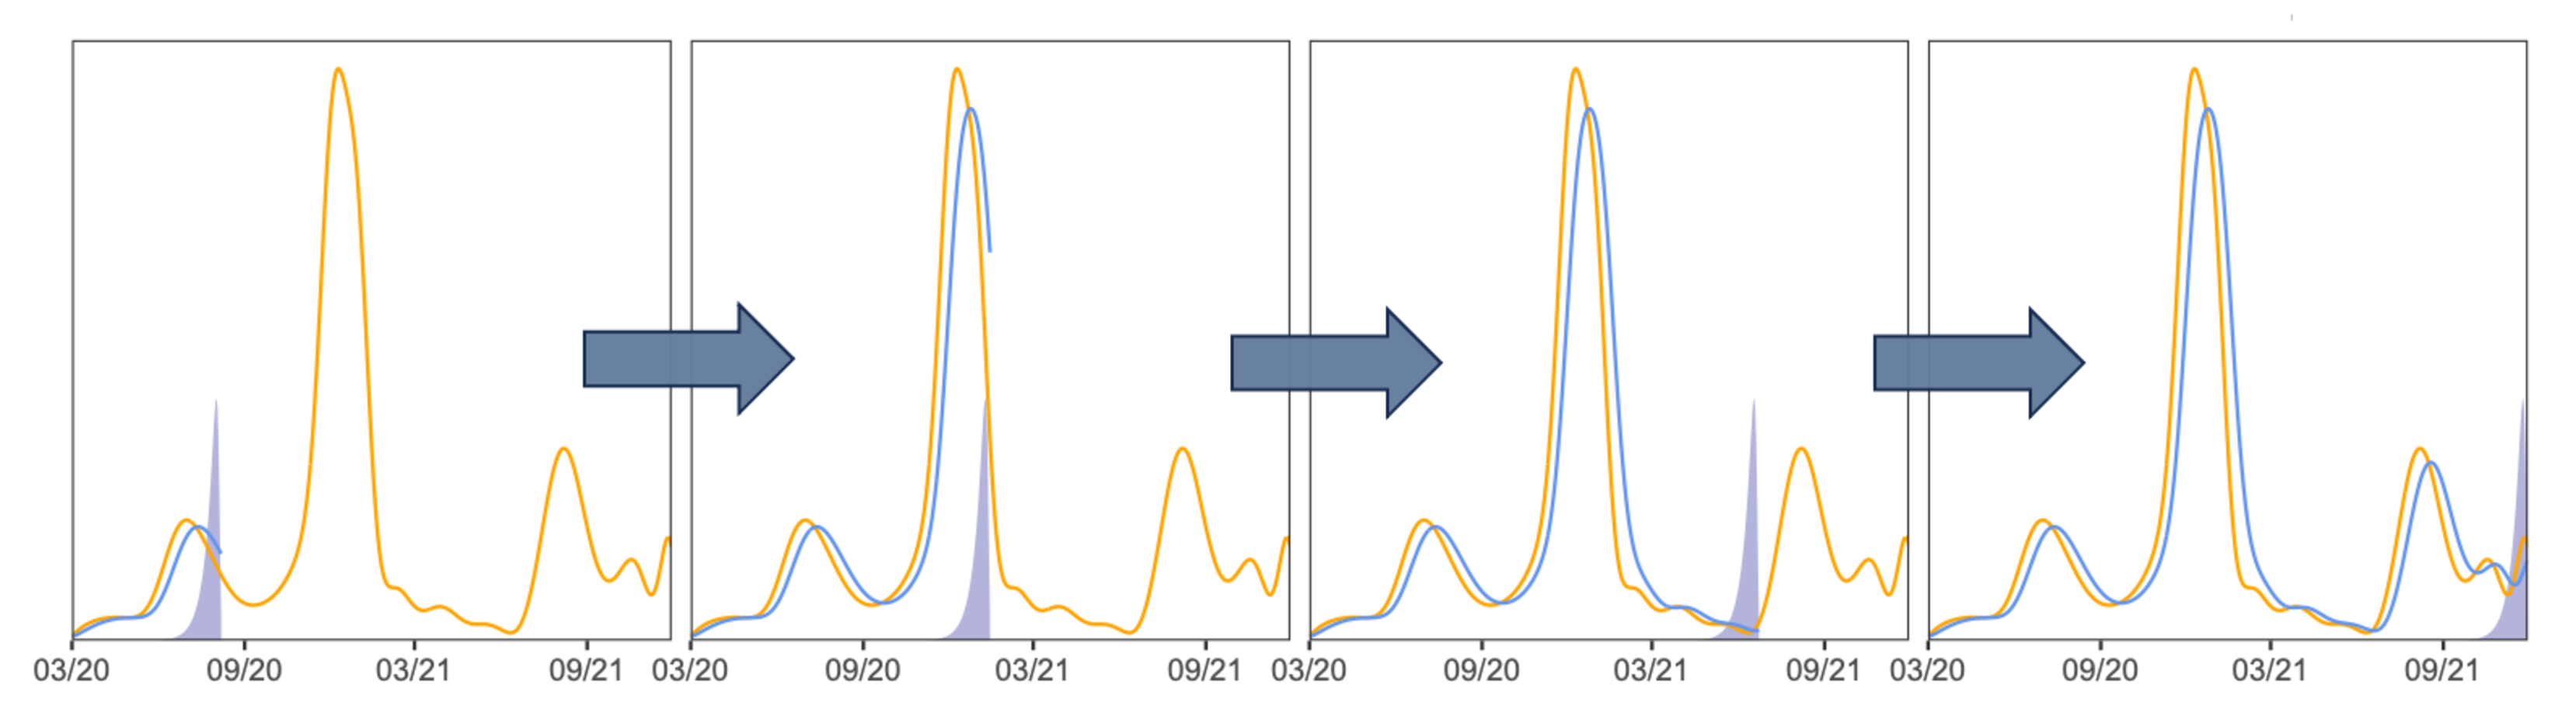
\includegraphics[width=0.99\linewidth]{convolution_diagram.pdf}
    \caption{A general depiction of convolving smoothed cases (orange line) with the corresponding delay probabilities (shaded blue area) to get the convolved estimates (blue line) over four different times.}
    \label{fig:convol}
\end{figure}

\subsection{Additional details on the date fields in the CDC line list}
\label{supp:linelist-details}

Because the CDC line list is updated monthly and cases may undergo revision, we
use a single version of it that was released on June 6, 2022. We consider this
version to be finalized in that it is well-beyond our study end date such that
the dataset is unlikely to be subject to further significant revisions.

\Cref{tab:order-events-table} presents the percent of pairwise occurrences for
the different possible permutations of events in the line list. Essentially,
most cases follow the idealized ordering shown by
\Cref{fig:chain_events_onset_report} and so we adhere to this construction as
much as possible. Unfortunately, the line list has significant missing data,
notably with respect to our variables of interest. Approximately 62.3\% of cases
are missing the symptom onset date, 55.4\% are missing positive specimen date,
and 8.96\% of cases are missing the report date. Furthermore, cases with missing
report or positive specimen dates may be filled with their symptom onset date
\citep{jahja2022real}. So it is possible that all three variables may have the
same date for a case. However, we only actually deal with pairs of these events;
we do not use all three at once in our construction of the delay distributions.
Therefore, we restrict our investigation of coincident missingness to the possible pairs.
% \Cref{fig:prop-cc} suggests that this issue impacts states differentially due to
% the inconsistent proportions of zero delay between positive specimen and report
% date across states. 

\begin{table}[t!]
    \centering
\begin{tabular}{@{}lp{3cm}p{8.5cm}@{}}
\toprule
\textbf{Order of events}& \textbf{Percent pairwise occurrence} &
\textbf{Handling}\\ \midrule \addlinespace
IO $\rightarrow$ SO $\rightarrow$ PS $\rightarrow$ RE & \begin{tabular}[t]{@{}l@{}}PS $\geq$ SO: 97.1 \\ PS = SO: 33.6\\ PS \textgreater\ RE: 1.74\\  PS = RE: 14.6\end{tabular} & This is the idealized order of events and so the  support sets for  SO $\rightarrow$ PS and PS $\rightarrow$ RE delay distribution constructions around this such that IO comes first by construction, SO typically precedes PS, but may be the same  or come before, and RE comes after PS and SO \\ \addlinespace
IO $\rightarrow$ PS $\rightarrow$ SO $\rightarrow$ RE & \begin{tabular}[t]{@{}l@{}}PS \textless\ SO: 2.91 \\ SO $\leq$ RE: 99.3 \\ SO \textless\ RE: 86.1\end{tabular}            & Allowed for negative delays up to the largest non-outlier value for the 0.05 quantile of delay from PS to SO by state                                                                                                                                         \\ \addlinespace
IO $\rightarrow$ PS $\rightarrow$ RE $\rightarrow$ SO & \begin{tabular}[t]{@{}l@{}}RE \textless\ SO: 0.7 \\ RE \textless\ PS: 1.7\end{tabular}                                    & Current handling by the CDC of the line list ensures that the most concerning cases are handled where SO = PO = RE, SO = RE and PO = RE                                                                                                                                                \\ \addlinespace\bottomrule
\end{tabular}
\caption{Percent pairwise occurrence for the different permutations of events considered in the restricted CDC line list. The abbreviation IO stands for infection onset, SO is symptom onset, PS is positive specimen, and RE is report date. We consider a restricted set of permutations because we assume that IO must come first and that PS must precede report date for a case to be legitimate. Finally, the underlying assumption for the percent pairwise occurrence calculations is that the cases must have both elements present (not missing).}
\label{tab:order-events-table}
\end{table}


Due to the contamination in the zero delay cases (those whose symptom onset was
used to fill missing positive specimen or report date, the true extent of which
is unknown to us), we omit all cases where the positive specimen and report
dates have zero delay from our analysis. We choose to allow for zero and
negative delay for symptom onset to report because correspondence with the CDC
confirms the possibility that a person could test positive before symptom onset
and it is a reasonable ordering to expect if, for example, the individual is
aware that they have been exposed to an infected individual.

\begin{figure}[!tb]
\centering
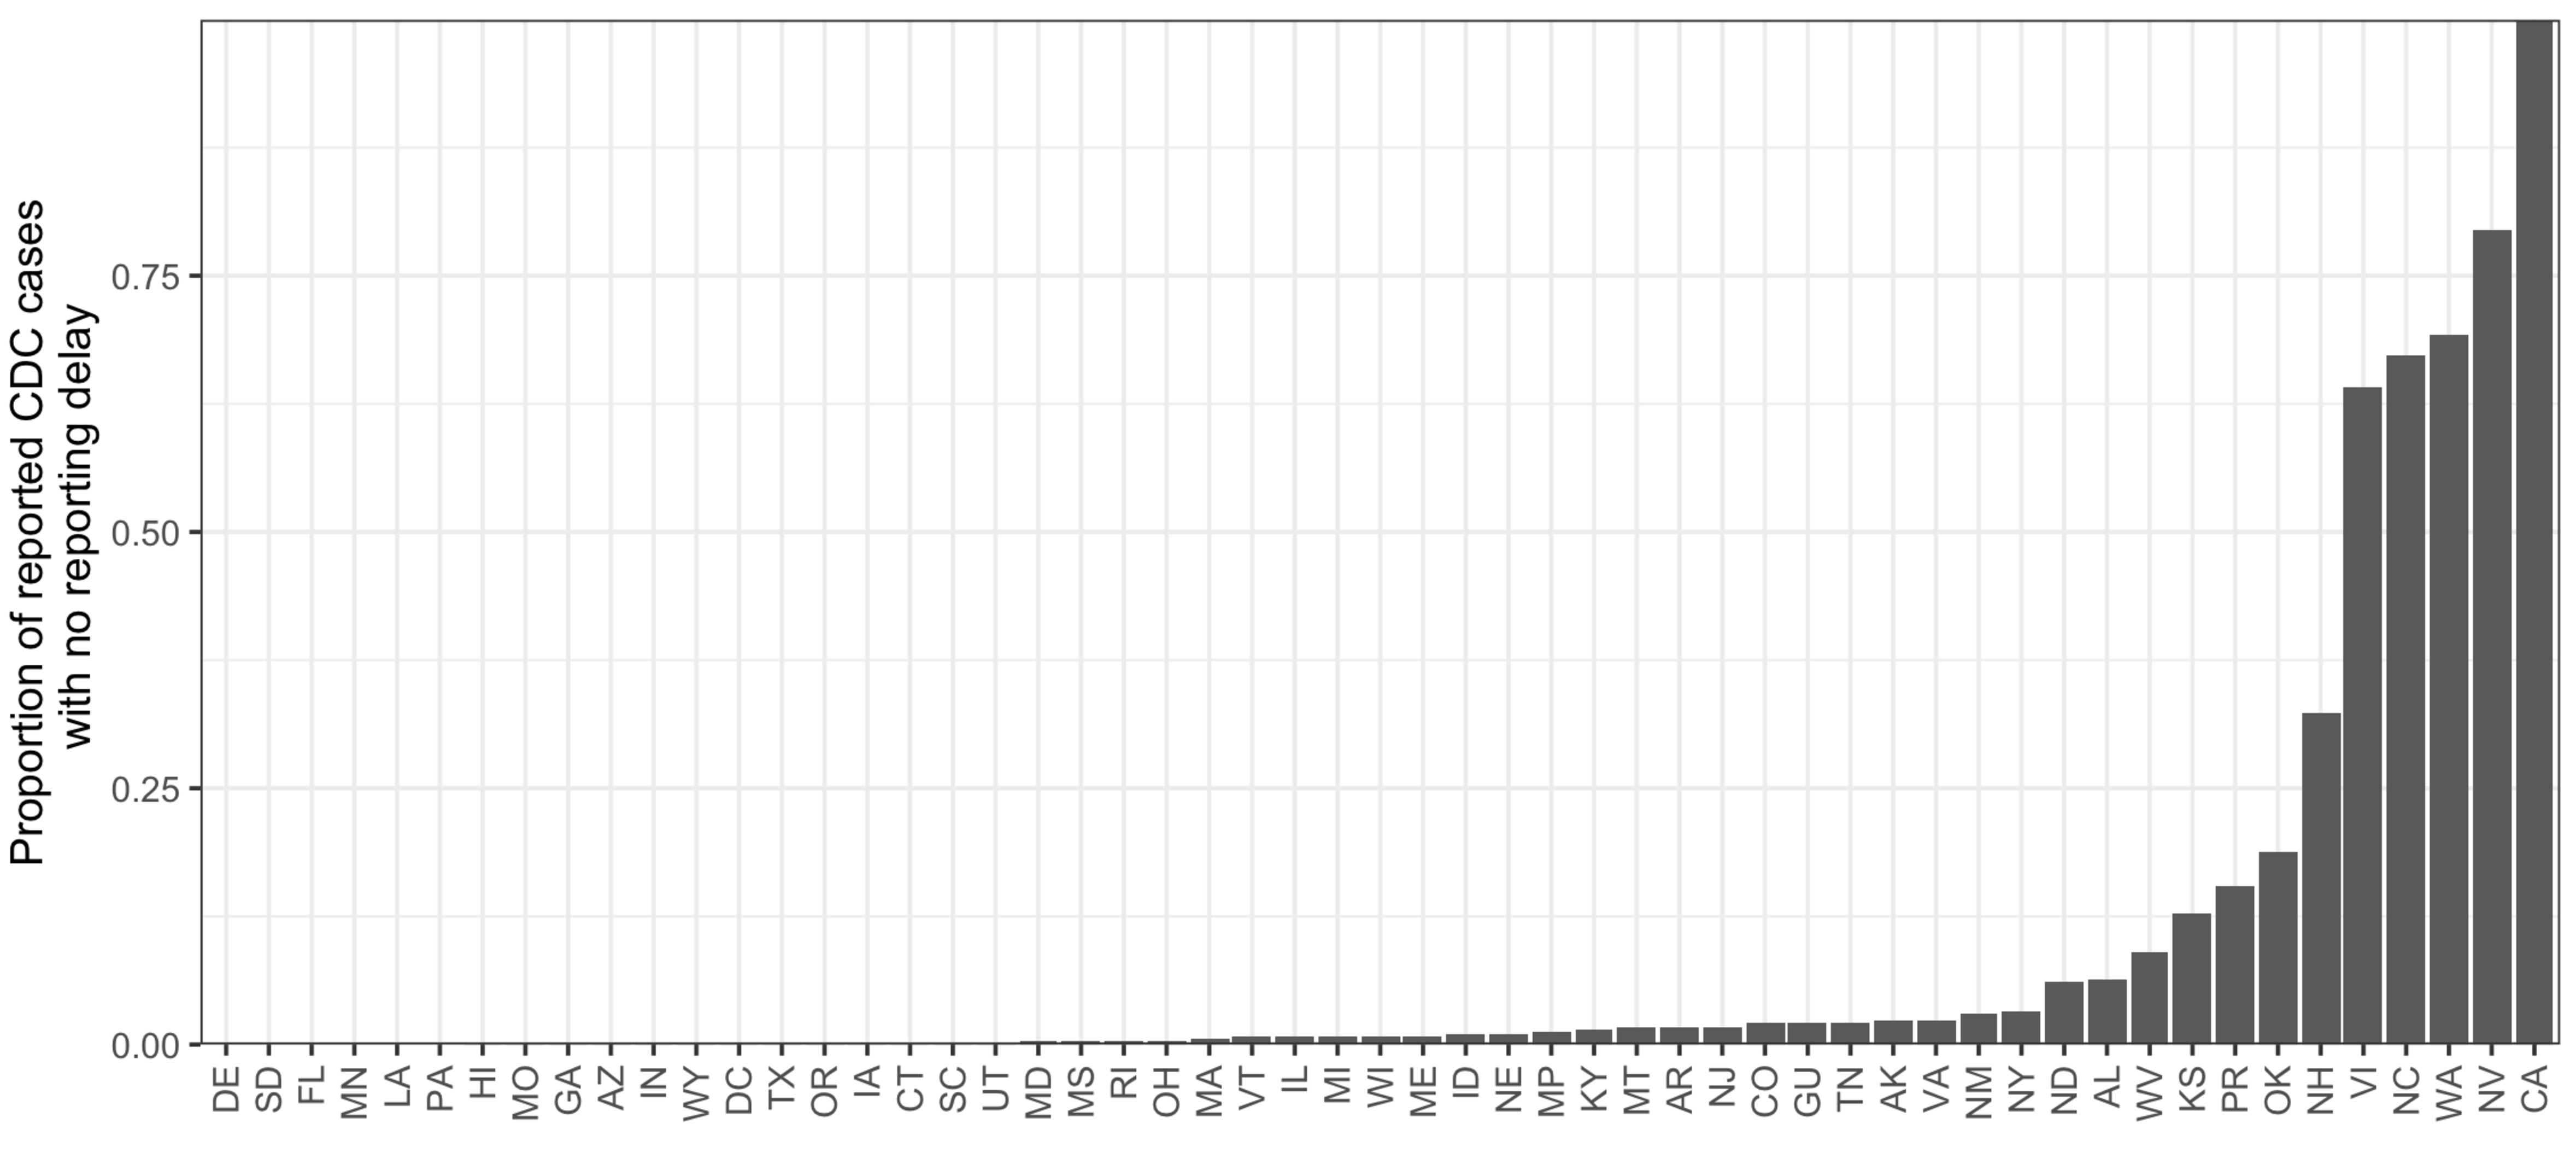
\includegraphics[width=0.9\linewidth]{prop_cc_zero_delay.pdf}\\
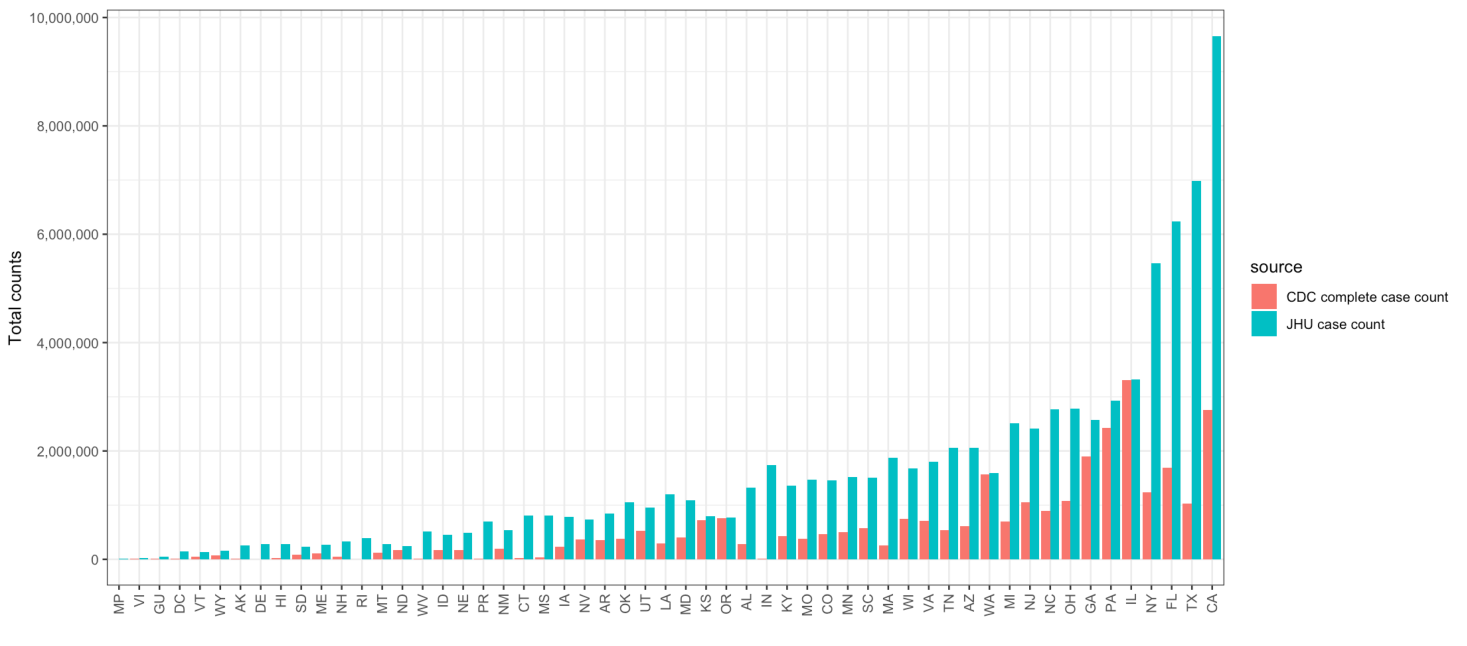
\includegraphics[width=0.9\linewidth]{prop_cc_cdc_vs_jhu.pdf} 
\caption{Top panel: Proportion of complete cases with zero delay between
    positive specimen and report date in the restricted CDC line list dataset.
    Bottom panel: Complete case counts by state in the CDC line list versus the
    cumulative complete case counts from JHU CSSE as of June 6, 2022. All
    counts have been scaled by the 2022 state populations as of July 1, 2022
    from \citep{uscensus2022annual}.}
\label{fig:prop-cc}
\end{figure}

The CDC restricted line list contains 74,849,225 cases (rows) in total compared
to 84,714,805 cases reported by the JHU CSSE; that is, line list is missing
about 10 million cases. The extent that this issue impacts each state is shown
in \Cref{fig:prop-cc}, from which it is clear the fraction of missing cases is
substantial for many states, often surpassing 50\% \citep{jahja2022real}. In
addition, the probability of being missing does not appear to be the same for
states, so there is likely bias introduced from using the complete case line
list data. We consider such bias to be unavoidable in our analysis due to a lack
of alternative line list sources. 



%\subsection{Table on the percent pairwise occurrence of events in the CDC line list}


\subsection{Additional details on delay distribution calculations}
\label{supp:delay-justifications}

In the line list, we observe unusual spikes in reporting in 2020 in comparison
to majority of 2021. When stratified by report date, a few states contribute
unusually large case counts on isolated dates very late in the reporting process
(well beyond 100 days following specimen collection). These large accumulations
of cases over time are likely due breakdowns of the reporting pipeline. Such
anomalies are not likely to be reliable indicators of the delay from positive
specimen to case report. Therefore, we prune these reporting backlogs
systematically. The heuristic is to find large batches of cases that were all
simultaneously reported on the same date with a lengthy delay (as would happen
if a state "found" a tranche of previously unreported positive tests).

For this, we operate only on part of the line list intended for the positive
specimen to case report delay estimation (as this is where we use case reports
from the line list). Then, we divide this line list into three roughly
evenly-spaced and non-overlapping intervals over 2020 and early 2021 (the
interval end points on July 16, 2020, October 16, 2020, and January 15, 2021).
For each interval, we separate the cases with reporting delays that are at least
50 days long into equally-sized bins of 50 days. Then, for each interval and
bin, we perform the following pruning procedure:
\begin{enumerate}[noitemsep]
\item Obtain the total count of these delays for each state. 
\item Check whether each such count on the log scale is at
least the median (for the bin) plus 1.5 times the interquartile range. Retain
only those that exceed this criterion as candidates for pruning. 
\item For the candidate states, compute the case counts by report date. 
\item If there is a report date for a candidate state with a case count greater 
than or equal to a pre-specified threshold, then remove/prune those cases from the line list. 
We set the threshold to be 2000 cases for the first two bins, and then lower
it to 500 for the remaining bins based on inspection.
\end{enumerate}

Finally, in New Hampshire, for a small handful of report dates, all cases
reported by JHU appear in the CDC line list, and all are recorded as having
positive specimen collection date equal to the report date. The resulting
estimate of the delay distribution (see \Cref{sec:step1})
$\widetilde{p}_{\textrm{NH},t}(k)$ would be a point mass at $k=0$ and the weight
$\alpha_{\textrm{NH},t}=1$ resulting $\widehat\pi_{\textrm{NH},t}(k)$ also being a
point mass at $k=0$. In this specific case, we force $\alpha_{\textrm{NH},t} =
\min_{\ell\neq\textrm{NH}} \alpha_{\ell,t}$.

\subsection{Variant circulation proportions}
\label{sec:variant-proportions}


To estimate the daily proportions of the variants circulating in each state, we
obtain the GISAID genomic sequencing data from CoVariants.org
\citep{hodcroft2021covariants, elbe2017data}. These counts represent the total
number of cases belonging to a particular variant using
a sample of positive tests over a biweekly period. To estimate the population
proportion of each variant, we apply multinomial logistic regression 
for the eight variant categories separately for each state. 
Multinomial logistic regression is a standard technique to model the
frequency of SARS-CoV-2 variants 
\citep{obermeyer2022analysis, annavajhala2021emergence, figgins2021sars}.

We let $V_{j\ell,t}$ to be the probability of a new cases at time $t$ in location
$\ell$ corresponding to variant $j$. Let $v_{j\ell,t}$ be the analogous observed
proportion. Then nonparametric multinomial logistic regression models the log odds
as the system
\begin{equation}
\log\left(\frac{V_{j\ell,t}}{1-V_{j\ell,t}}\right) = \beta_{j\ell,0} + \beta_{j\ell,1} t + \beta_{j\ell,2}t^2 + \beta_{j\ell,3}t^3,\;\; j=1,\ldots J.
\end{equation}
This is estimated along with a constraint to ensure that the estimated proportions will sum to 1 across all
$J$ variants. The specification of the log odds as a third-order polynomial in
time produces smoothness of the estimated proportions.
 \Cref{fig:prop_figs} shows the proportions by variant for California before
(left) and after (right) the smoothing procedure. 

\begin{figure}[!tb]
    \centering
        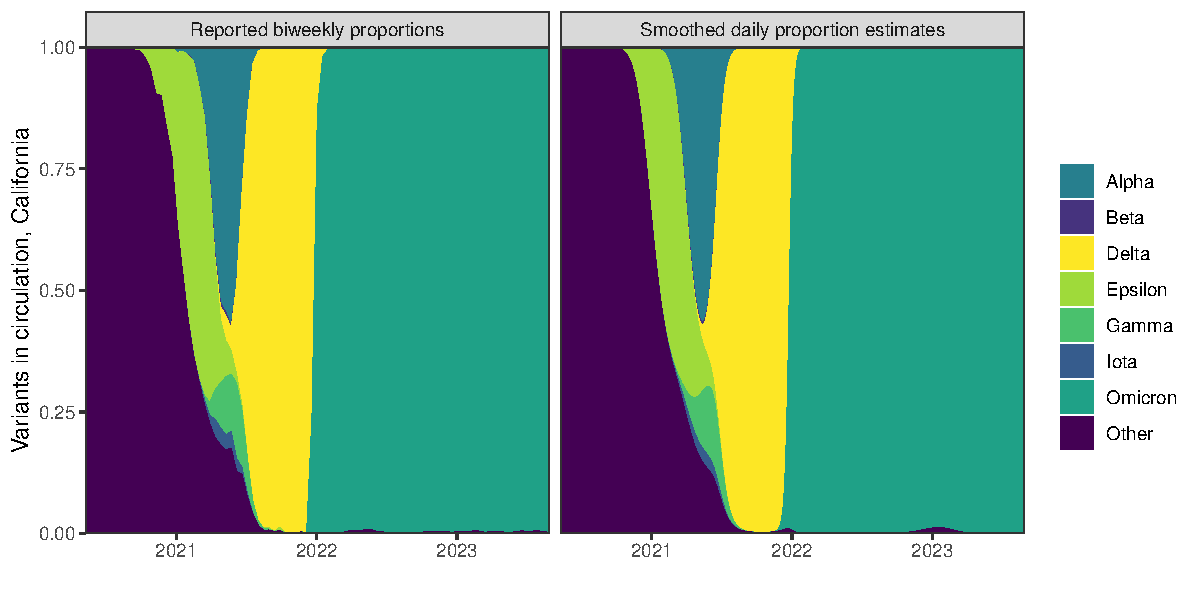
\includegraphics[width=\linewidth]{var-props-1.pdf}
        \caption{Left: Original biweekly proportions of the variants in circulation
        for California. Right: Daily proportions of the variants in circulation for
        California.}
        \label{fig:prop_figs}
    \end{figure}


    


\subsection{Constructing the delay from infection to test}
\label{supp:delay-sops}

The result of Step 1 (\Cref{sec:step1}) is $\widehat{x}_{\ell,t}$, case
estimates by positive specimen date for each state. To continue, pushing this
back to infection estimates, we need the variant-specific delays from infection
to positive specimen collection. As shown in \Cref{fig:chain_events_onset_report}, this delay can be broken into two separate pieces: (1) the
delay from infection to symptom onset, and (2) the delay from symptom onset to
positive specimen collection. The first requires different methods and is
specific to the variant causing the infection, while the second is estimable from the CDC line
list.

\subsubsection{Estimating the incubation period distributions} 
\label{sec:incubation}

To account for the incubation period, the time between infection and symptom
onset, we use estimates from the existing literature, modified slightly for
coherence with each other: we model each incubation as a gamma distribution with
different parameters. We focus on the following eight variants (shown in
\Cref{fig:prop_figs}), which saw significant circulation in one of the \US states
during our study period: Ancestral/Other, Alpha, Beta, Epsilon,
Iota, Gamma, Delta, and Omicron. Alpha, Beta, Delta, Gamma, and Omicron are all
variants of concern \citep{who2021tracking}, while we include the Epsilon
(California) and Iota (New York) variants because of large impact on those and
neighbouring states \citep{yang2022investigation, duerr2021dominance}.

The incubation period of the Ancestral variant has been modelled as a gamma
distribution \citep{tindale2020evidence}, so we simply use the reported shape
and scale parameters. For the Alpha, Beta, Gamma, Delta and Omicron variants,
the mean and standard deviation are reported \citep{tanaka2022shorter,
grant2022impact, ogata2022shorter}. Therefore, we use method of moments to match
the mean and variance to estimate the gamma parameters, using the moment
equations given in \Cref{sec:step1}. Then, we discretize each resulting density
shown in \Cref{fig:inc_gammas} to the support set, which is taken to be from 1
and 21 days. This range assumes that symptoms require at least 1 day to develop
\citealp{phcan2021covid} and that an asymptomatic infection will resolve within
21 days \citep{zaki2021estimations,cortes2022sars}.

We were unable to locate incubation period estimates for the geo-specific
Epsilon and Iota variants, so we use the incubation period for Beta because
Epsilon, Iota, and Beta are all children from the same parent in the
phylogenetic tree of the Nextstrain Clades \citep{hodcroft2021covariants}. All
other circulating variants are grouped together with the Ancestral variant.
There was little available sequencing data prior to Alpha-emergence, but
unfortunately, later in the pandemic, it is impossible to separate Ancestral
from other rare variants, though these also saw minimal circulation after
the middle of 2021.

\begin{figure}[!tb]
\centering
    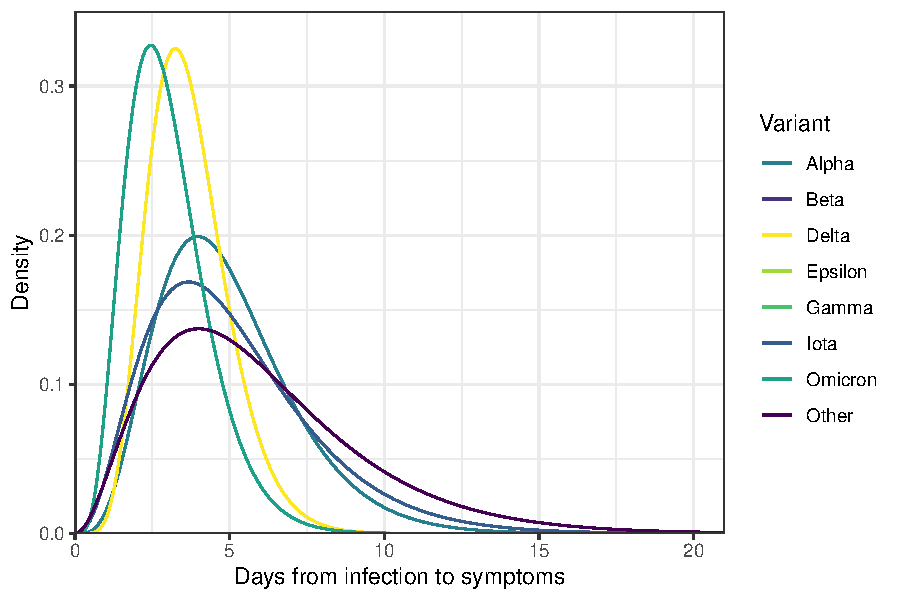
\includegraphics[width=0.6\linewidth]{inc-gammas-1.pdf}
    \caption{Gamma density for the incubation period of each of the eight
    variant categories. Note that the Ancestral variant uses reported shape and
    scale parameters \citep{tindale2020evidence}, while the remaining variants
    convert reported estimates for the mean and variance
    \citep{tanaka2022shorter,grant2022impact,ogata2022shorter} using the method
    of moments to produce the gamma parameters.}
    \label{fig:inc_gammas}
\end{figure}





\subsubsection{Estimating the delay distributions for symptom onset to positive specimen}
\label{supp:delay-sops}


Estimating the delay from symptom onset to positive specimen date follows a
similar procedure as described in \Cref{sec:step1} with a minor
adjustment. Here, we allow $k$ to range from $-3$ to $21$ (rather than $1$ to
$60$). These upper and lower bounds are based on the largest delay values for
the state-wide 0.05 and 0.95 quantiles. The median
delay is very short at approximately 2 days, and an asymptomatic individual may
test positive following a known exposure, before the onset of symptoms. We show
both types of delays for a sample of states over several dates in
\Cref{fig:delay-plots-samp}. Unlike the delay from positive specimen collection
to report, the delay from symptoms to positive specimen can conceivably be
negative. The most obvious reason for this would be if a person knew they had been
exposed to an infectious individual and so got tested prior to the development
of symptoms. Required regular testing for jobs in health care settings,
construction, or the film industry could also produce negative delays.


\begin{figure}[t!]
\centering
    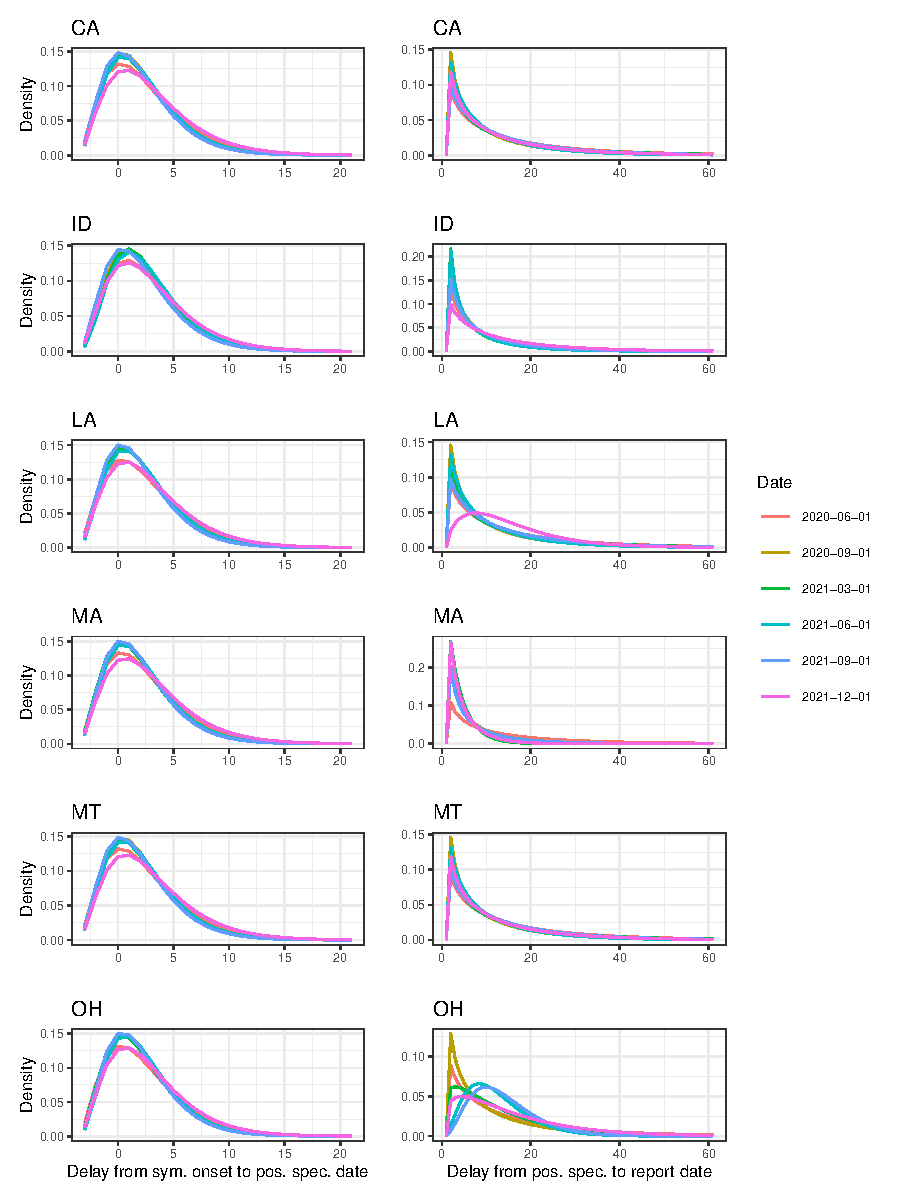
\includegraphics[width=.90\textwidth]{delay_plots.pdf} 
    \caption{Depictions of the estimated delay from symptom onset to
    positive specimen date (left) and from positive specimen date to report date
    (right) for a sample of six states over several dates.}
    \label{fig:delay-plots-samp}
\end{figure}

\subsubsection{Details on constructing the infection-to-test distributions}
\label{supp:details-conv}

Finally, to produce the delay from infection to positive specimen collection we
convolve the variant-specific incubation periods from \Cref{sec:incubation},
denoted by $\{i_{j}(k) : 0 < k \leq 21\}$ with the location-time-specific
symptom-to-positive-test distributions from \Cref{supp:delay-sops}, denoted by
$\{q_{\ell,t}(k) : -3\leq k \leq 21\}$. The convolution of these yields a
distribution $\{\tau_{j\ell,t}(k): -3 \leq k
\leq 42\}$. \Cref{fig:delay-plots-samp} shows the delays used for a sample of 6
states: symptom to positive specimen (left column) and positive specimen to report
(right column). The convolution distribution $\tau_{j\ell,t}$ requires
convolving the distribution in the left column with the variant-specific
incubation periods shown in \Cref{fig:inc_gammas}.





\subsection{Details about seroprevalence data}
\label{supp:sero-details}

We use two major contemporaneous surveys to estimate the proportion of the
population with evidence of previous infection in each state over time: the
2020--2021 Blood Donor Seroprevalence Survey and the Nationwide Commercial Lab
Seroprevalence Survey \citep{cdc2021blood, cdc2021comm}. In the former, the CDC
collaborated with 17 blood collection organizations in the largest nationwide
COVID-19 seroprevalence survey to date \citep{cdc2021blood}. The blood donation
samples were used to construct monthly seroprevalence estimates for nearly all
states from July 2020 to December 2021 \citep{jones2021estimated}. In the latter
survey, the CDC collaborated with two private commercial laboratories to test
blood samples from people that were in for routine or clinical management
(presumably unrelated to COVID-19 \citealp{bajema2021estimated}) for the
antibodies to the virus. The resulting dataset contains seroprevalence estimates
for a number of multi-week collection periods starting in July 2020 to February
2022. 

Both datasets are based on repeated, cross-sectional studies that estimate the
percentage of people who were previously infected with COVID-19 using the
percentage of people from a convenience sample who had antibodies against the
virus \citep{bajema2021estimated, cdc2020data, jones2021estimated}. Adjustments
were made in both for age and sex to account for the demographic differences
between the sampled and the target populations. However, both datasets are
incomplete and they differ in the number and the timing of the data points for
each state (\Cref{fig:sero-blood-comm-compar}). For example, in the
commercial dataset, the last estimate for North Dakota is in September 2020. In
the blood donor dataset, Arkansas does not have estimates available until
October 2020. 

\begin{figure}[!tb]
\centering
    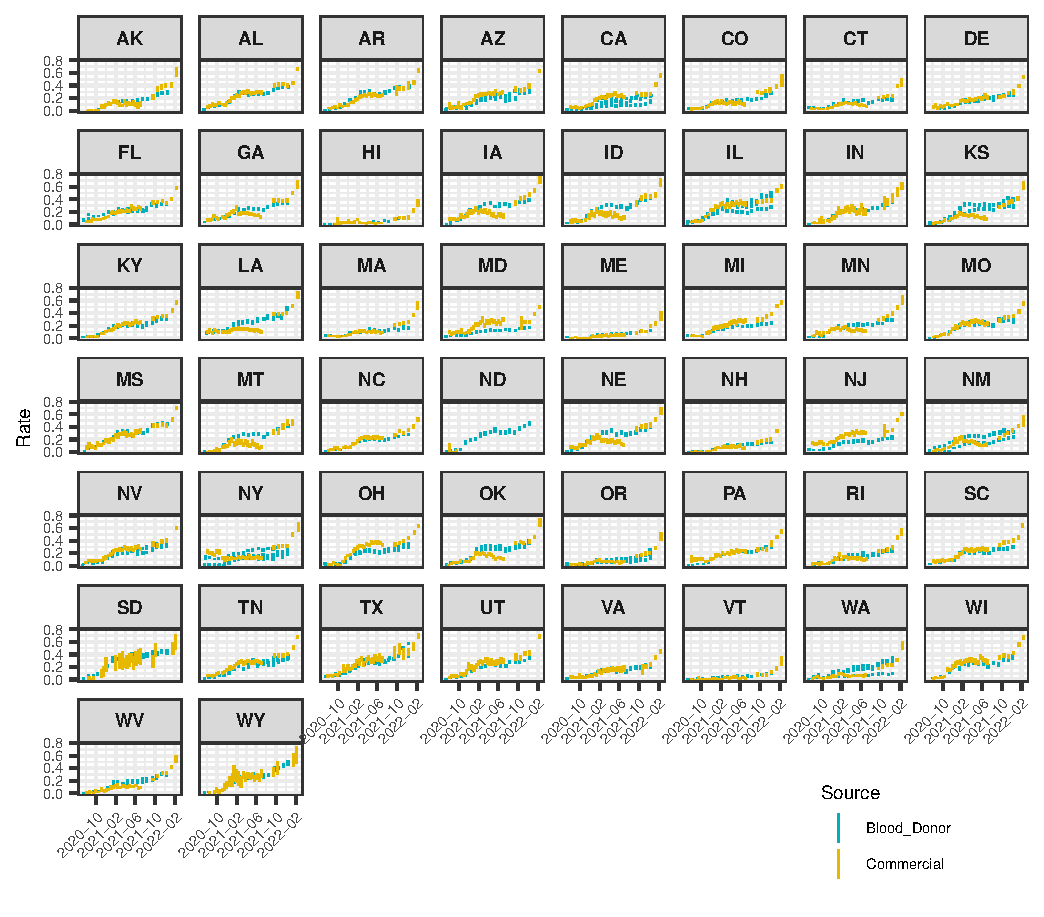
\includegraphics[width=.99\textwidth]{sero_blood_comm_compar.pdf}
    \caption{A comparison of the seroprevalence estimates from the Commercial
    Lab Seroprevalence Survey dataset (yellow) and the 2020--2021 Blood Donor 
    Seroprevalence Survey dataset (blue). Note that the maximum and the minimum
    of the line ranges are the provided 95\% confidence interval bounds to 
    give a rough indication of uncertainty.}
    \label{fig:sero-blood-comm-compar}
\end{figure}
    
A major difference in the structure of the two datasets is that the commercial
dataset always has the seroprevalence estimates at the level of the state, while
the blood donor dataset can either have estimates for the state or for multiple
separate regions within the state. For the commercial dataset, we use the
midpoint of the provided specimen collection date variable.  For the blood donor
dataset, we use the median donation date if the seroprevalence estimates are
designated to be for entire state. If they are instead for regions in the state,
since there is reliably one measurement per region per month, we aggregate the
measurements into one per month per state by using a weighted average (to
account for the given sample sizes of the regions). The median of the median
dates is taken to be the date for the weighted average. If there are multiple
measurements in a week from a seroprevalence source, then the average is used.


\subsection{State space representation of the antibody prevalence
model}\label{supp:ssapm} 

The antibody prevalence model described in \Cref{sec:report-ratio} can be expressed
as a linear Gaussian state space model \citep{durbin2012time}.
For $m = 1, \dots, M$, let $\alpha_m$ be a vector of
latent state processes at time $m$ and $y_m$ be a vector of
observations at time $m$. The form of the (general) linear Gaussian state space model is 
\begin{align}
y_m &= Z\alpha_m + \sigma^2_r\epsilon_m, \qquad \epsilon_m \sim N(0, H_m) \label{eq:ss1}\\
\alpha_{m+1} &= T_m\alpha_m + R\eta_m, \quad \eta_m \sim N(0, Q) \label{eq:ss2}
\end{align}
where $\alpha_1 \sim N(a_1, P_1)$ and 
$\epsilon_m$ and $\eta_m$ are mutually and serially independent.

% Kalman filtering gives the following one-step-ahead predictions of the states
% \begin{align*}
% a_{t+1} &= \E[\alpha_{t+1}\given y_t, \dots, y_1] 
% \end{align*} with covariance,
% \begin{align*}
% P_{t+1} &= \Var(\alpha_{t+1} \given y_t, \dots, y_1).
% \end{align*}
% Then, the Kalman smoother works backwards to the first time to give
% \begin{align}
% \hat{a}_t &= \E[\alpha_{t}\given y_n, \dots, y_1] \label{eq:hatat}\\
% V_t &= \Var(\alpha_{t}\given y_n, \dots, y_1). \label{eq:Vt}
% \end{align}
% The filtering and smoothing steps are based on recursions that are described in
% Appendix A of \citep{helske2017kfas} as we use the R package KFAS to estimate
% our model.

% For our situation, the Kalman filter and smoothing approach offers a number of
% advantages over the penalized regression approach. Perhaps most notably,
% the parameters are estimated all at once (so cross validating for model
% parameter tuning is not necessary). Another major benefit is that it can handle 
% unevenly spaced time series (refer to \citealp{durbin2012time} for further details).

To express the antibody prevalence model in state space form, we relate the
model in \Crefrange{eq:sero-measurements}{eq:report-ratio} to the components in
\Cref{eq:ss1,eq:ss2} as follows (omitting the location subscript for
simplicity):

% Probably move the below specification to the appendix

\begin{align*}
    Z &= \begin{bmatrix} 1 & 0 & 0 & 0 \\ 0 & 1 & 0 & 0 \end{bmatrix} &
    H_m &= \begin{bmatrix}w^1_{m} & 0 \\ 0 & w^2_{m} \end{bmatrix} \\
    \alpha_m &= \begin{bmatrix}s_{m} \\ a_m \\ a_{m-1}\\ a_{m-2} \end{bmatrix} & 
    T_m &= \begin{bmatrix}(1 - \gamma) & \widehat{u}^\Sigma_{m} (1 - z_m) & 0 & 0\\ 
        0 & 3 & -3 & 1 \\ 0 & 1 & 0 & 0\\ 0 & 0 & 1 & 0 \end{bmatrix}  & 
    R &= \begin{bmatrix}1 & 0  \\ 0 & 1 \\ 0 & 0 \\ 0 & 0 \end{bmatrix}\\
    Q &= \begin{bmatrix} \sigma^2_\epsilon & 0  \\ 0 & \sigma^2_\eta \end{bmatrix} &
    a_1 &= \begin{bmatrix} \tilde{s}_{1}\\ \tilde{a}_1\\ \tilde{a}_1 \\ \tilde{a}_1 \end{bmatrix} & 
    P_{1} &= \begin{bmatrix} \sigma^2_{\tilde{s}_{1}} & 0 & 0 & 0 \\ 
    0 & \sigma^2_{\tilde{a}_1} & 0 & 0\\ 0 & 0 & \sigma^2_{\tilde{a}_1} & 0 \\ 
    0 & 0 & 0 & \sigma^2_{\tilde{a}_1} \end{bmatrix} 
\end{align*}
where $\sigma^2_r$ is the variance of observations, $\sigma^2_\epsilon$ is the
variance of the seroprevalence estimates, $\sigma^2_\eta$ is the trend variance,
and $\widehat{u}^\Sigma_{m}$ denotes the new deconvolved cases between $m$ and
$m+1$. Because the inverse reporting ratios should be more variable than the
seroprevalence estimates, we enforce that the estimate of $\sigma^2_\eta$ is a
multiple of $\sigma^2_\epsilon$. 

Finally, $w^1_{m}$ and $w^2_{m}$ are the time-varying inverse variance weights
computed from the commercial and blood donor datasets, respectively. For each
source, we compute the weights for the observed seroprevalence estimates using
the formula for the standard error of a proportion. These weights are then
re-scaled to sum to the number of observed seroprevalence measurements for the
source. Finally, the ratio of the average observed weights from the two sources
is used to scale all weights relative the commercial source. This transformation
is done purely for computational purposes to make estimation of the unknown
parameters easier.

The prior distribution for $\alpha_1$ is estimated using both data-driven
constraints and externally sourced information. The initial value of the
seroprevalence component, $\tilde{s}_{1}$ is the average of the initial
seroprevalence measurements from each source rounded down to two decimal places,
The corresponding initial variance estimate, $\sigma^2_{\tilde{s}_{1}}$, is
taken to be the mean of the standard errors of the two seroprevalence estimates.
For the initial values of the trend components, we use the inverse of the
ascertainment ratio estimate for each as of June 1, 2020 from Table 1 in
\citep{unwin2020state}: the mean for $\tilde{a}_1$ and half the width of the
confidence interval converted to the inverse for
$\sigma^2_{\tilde{a}_1}$.

The initial $\sigma^2_r$ is taken to be the average of the estimated variances
from the observed seroprevalence measurements regressed linearly on time.
The initial value of the multiplier is set to be $100$ for all states. The
$\sigma^2_\epsilon$ and $\gamma$ values are estimated separately for each state,
then fixed to their averages on the log-scale.

Following maximum likelihood estimation of remaining parameters we use the
Kalman filter to obtain the smoothed point estimates and variances of the weekly
inverse reporting ratios. We use forward and backward extrapolation to extend
these estimates outside of the observed seroprevalence range
\citep{durbin2012time}, followed by linear interpolation to produce daily
values. We then multiply these by the
corresponding deconvolved case estimates before converting to per-capita values.
Annual estimates of the state
populations as of July 1 of 2020 are taken from the Dec.\
2022 press release from the \US Census Bureau \citep{uscensus2022annual}.


% The $50$, $80$, and $95\%$ confidence intervals are constructed by taking a
% Bayesian view of the antibody prevalence model (refer to \ref{supp:bayeswaning} 
% for the Bayesian specification of the model). 
% That is, for each time, $t$, we obtain an estimate of the
% posterior variance of $a_t$, apply the deconvolved case estimate as a constant
% multiplier, and then use resulting variance to build a normal confidence
% interval about the infection estimate. We additionally enforce that the lower
% bound must be at least the deconvolved case estimate for the time under consideration.


% \subsection{Bayesian specification of the antibody prevalence
% model}\label{supp:bayeswaning} 
% In brief, the antibody prevalence model where we let
% $\beta = \left \{  \gamma, a_1,\dots, a_t \right \}$ and $X$ be the design
% matrix, corresponds to a Bayesian model with prior 
% \begin{align*}
%     \beta \sim N \left( 0,  \frac{\sigma^2 }{ \lambda} \left( A^TD^TDA 
%     \right)^{-1}  \right)
% \end{align*} and likelihood 
% \begin{align*}
%     s|X,\beta \sim N \left( X\beta, \sigma^2W^{-1} \right),
% \end{align*} where $A$ is indicator matrix save for the first column of $0$s 
% (corresponding to $\gamma$), $D$ represents the discrete derivative matrix of 
% order $3$, and $W$ is the inverse variance weights matrix. Then, the posterior 
% on $a_t$ is normally distributed with mean 
% \begin{align*}
%     \left ( X^TWX + \lambda A^TD^TDA \right )^{-1}X^TWs
% \end{align*} 
% and variance 
% \begin{align*}
%     \sigma^2 (X^TWX + \lambda A^TD^TDA)^{-1}.
% \end{align*}


% \subsection{Scaling by population}



% \subsection{Ablation analysis of infection-hospitalization correlations}

% To better understand the contribution of the intermediate steps to the lagged
% correlation analysis, we carry out a brief ablation study in which we calculate
% the lagged correlation using the following infection estimates: 1. those from
% the deconvolution procedure under the assumption that the infection onset is the
% same as the positive specimen date (i.e., excluding the positive specimen to
% infection onset data and deconvolution); 2. those from the deconvolution
% procedure under the assumption that the infection onset is the same as the
% symptom onset date (excluding the incubation period data); 3. those from the
% deconvolution procedure when utilizing all incubation period and delay data (the
% deconvolved case estimates); 4. those from applying the antibody prevalence
% model to produce estimates for both the reported and the unreported cases (the
% infection estimates).

% The results of this study are shown in \Cref{fig:abl-lag-cor}. From
% this, we can see that the deconvolved case and infection estimates from the
% intermediate steps are all leading indicators of hospitalizations. However, the
% degree that each such set of estimates lead hospitalizations depend on its
% location in the sequence of deconvolution steps and how close the estimates are to infection
% onset. For example, the deconvolved cases by positive specimen date tend to
% precede hospitalizations by about $11$ days, while those for the subsequent step
% indicate that the deconvolved cases by symptom onset tend to precede
% hospitalizations by a longer time of $13$ days. Finally, after adding the
% variant-specific incubation period data into the deconvolution and obtaining the
% deconvolved case estimates, we can observe that the reported infections precede
% hospitalizations by about $19$ days. 

% \begin{figure}[H]
% \centering
%     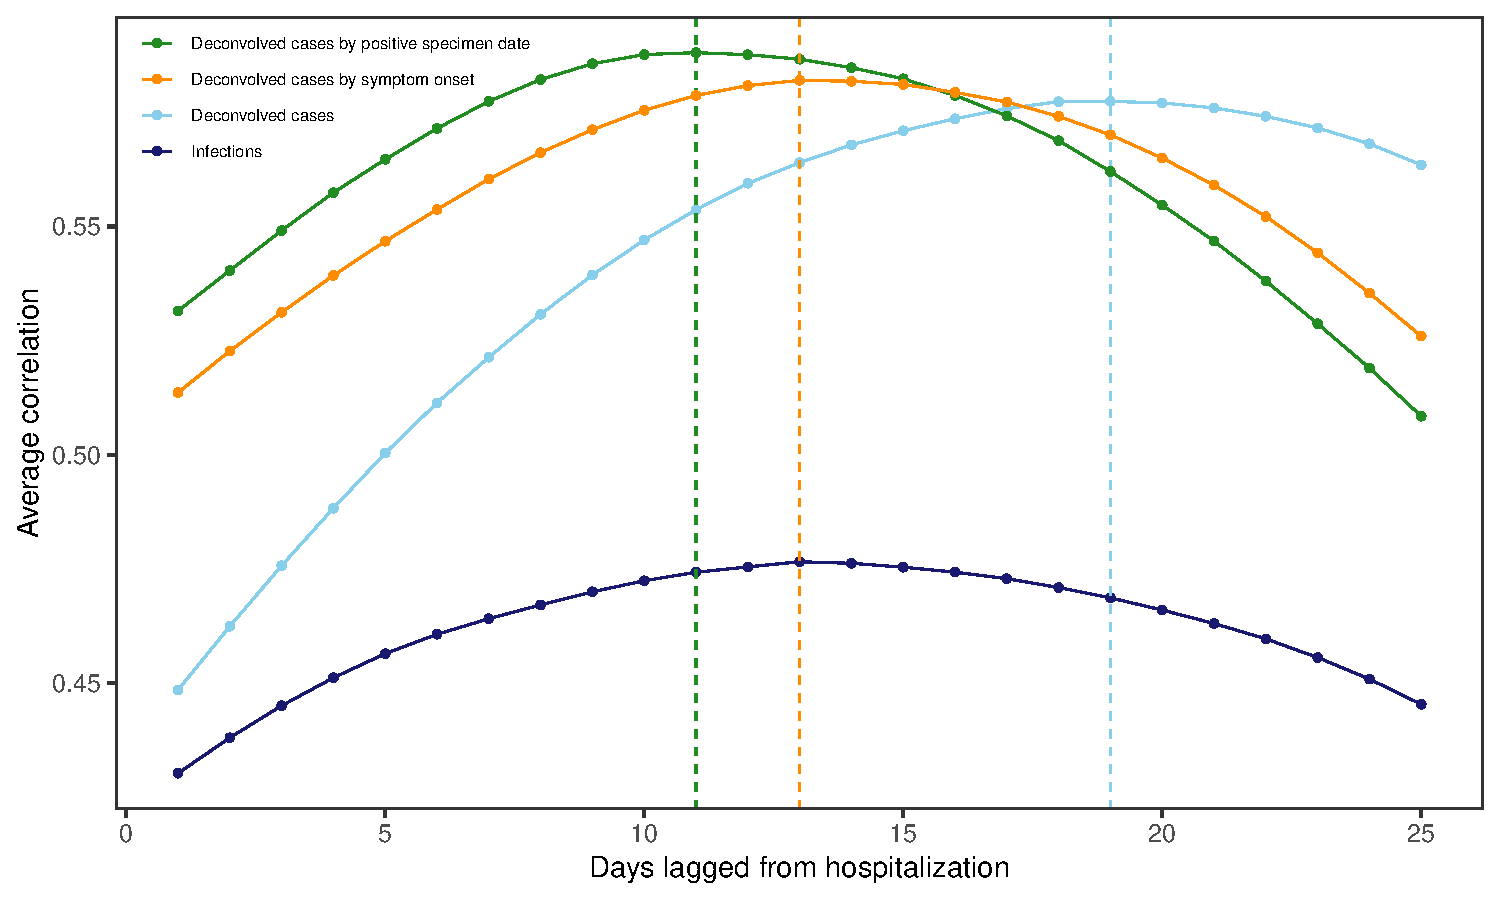
\includegraphics[width=.78\textwidth]{adj_unadj_pi_no_inc_hosp_lag_corr_F24.pdf} 
%     \caption{Lagged Spearman's correlation between the infection and
%     hospitalization rates per 100,000 averaged for each lag across \US states
%     and days over June 1, 2020 to November 29, 2021, and taken over a rolling
%     window of 61 days. The infection rates are based on the counts for the
%     deconvolved case and infection estimates as well as the reported infections
%     by symptom onset and when the report is symptom onset. Note that each such
%     set of infection counts is subject to a center-aligned 7-day averaging to
%     remove spurious day of the week effects. The dashed lines indicate the lags
%     for which the highest average correlation is attained.}
%     \label{fig:abl-lag-cor}
% \end{figure}
 

\end{document}